
\subsection{Кр 1 базовый поток, }


\begin{enumerate}
\item  Из семей, имеющих двоих разновозрастных детей, случайным образом выбирается одна семья. Известно, что в семье есть девочка (событие $A$).

\begin{enumerate}
\item	Какова вероятность того, что в семье есть мальчик (событие $B$)?

\item	Сформулируйте определение независимости событий и проверьте, являются ли события $A$ и $B$ независимыми?
\end{enumerate}

\item  Система состоит из $N$ независимых узлов. При выходе из строя хотя бы одного узла, система дает сбой. Вероятность выхода из строя любого из узлов равна 0.000001. Вычислите максимально возможное число узлов системы, при котором вероятность её сбоя не превышает 0.01.

\item  Исследование состояния здоровья населения в шахтерском регионе «Велико-кротовск» за пятилетний период показало, что из всех людей с диагностированным заболеванием легких, 22\% работало на шахтах. Из тех, у кого не было диагностировано заболевание легких, только 14\% работало на шахтах. Заболевание легких было диагностировано у 4\% населения региона.

\begin{enumerate}
\item	Какой процент людей среди тех, кто работал в шахте, составляют люди с диагностированным заболеванием легких?

\item	Какой процент людей среди тех, кто НЕ работал в шахте, составляют люди с диагностированным заболеванием легких?
\end{enumerate}

\item  Студент Петя выполняет тест (множественного выбора) проставлением ответов наугад. В тесте 17 вопросов, в каждом из которых пять вариантов ответов и только один из них правильный. Оценка по десятибалльной шкале формируется следующим образом:
\[
    \text{Оценка} = \left\{
                      \begin{array}{ll}
                        \text{ЧПО} - 7, & \text{если $\text{ЧПО}\in [8;\,17]$,} \\
                        1,              & \text{если $\text{ЧПО}\in [0;\,7]$,}
                      \end{array}
                    \right.
\]
где ЧПО означает число правильных ответов.

\begin{enumerate}
\item	Найдите наиболее вероятное число правильных ответов.

\item	Найдите математическое ожидание и дисперсию числа правильных ответов.

\item	Найдите вероятность того, что Петя получит «отлично» (по десятибалльной шкале получит 8, 9 или 10 баллов).

Студент Вася также выполняет тест проставлением ответов наугад.

\item	Найдите вероятность того, что все ответы Пети и Васи совпадут.
\end{enumerate}

\newpage
\item  Продавец высокотехнологичного оборудования контактирует с одним или двумя потенциальными покупателями в день с вероятностями 1/3 и 2/3 соответственно. Каждый контакт заканчивается «ничем» с вероятностью 0.9 и покупкой оборудования на сумму в 50\,000 у.\,е. с вероятностью 0.1. Пусть $\xi$ — случайная величина, означающая объем дневных продаж в у.\,е.

\begin{enumerate}
\item	Вычислите  $\P(\xi = 0)$.

\item	Сформулируйте определение функции распределения и постройте функцию распределения случайной величины $\xi$.

\item	Вычислите математическое ожидание и дисперсию случайной величины $\xi$.
\end{enumerate}


\item  Интервал движения поездов метро фиксирован и равен $b$ минут, т.\,е. каждый следующий поезд появляется после предыдущего ровно через $b$ минут. Пассажир приходит на станцию в случайный момент времени. Пусть случайная величина $\xi$, означающая время ожидания поезда, имеет равномерное распределение на отрезке $[0; \, b]$.

\begin{enumerate}
\item Запишите плотность распределения случайной величины $\xi$.

\item	Найдите константу $b$, если известно, что в среднем пассажиру приходится ждать поезда одну минуту, т.\,е. $\E(\xi) = 1$.

\item	Вычислите дисперсию случайной величины $\xi$.

\item	Найдите вероятность того, что пассажир будет ждать поезд менее одной минуты.

\item	Найдите квантиль порядка $0.25$ распределения случайной величины $\xi$.

\item	Найдите центральный момент порядка 2017 случайной величины $\xi$.

\item	Постройте функцию распределения случайной величины $\xi$.

Марья Ивановна из суеверия всегда пропускает два поезда и садится в третий.

\item	Найдите математическое ожидание и дисперсию времени, затрачиваемого Марьей Ивановной на ожидание «своего» поезда.

Глафира Петровна не садится в поезд, если видит в нем подозрительного человека. Подозрительные люди встречаются в каждом поезде с вероятностью $3/4$.

\item	Найдите вероятность того, что Глафире Петровне придется ждать не менее пяти минут, чтобы уехать со станции.

\item	Найдите математическое ожидание времени ожидания «своего» поезда для Глафиры Петровны.
\end{enumerate}

\item  (Бонусная задача) На первом этаже десятиэтажного дома в лифт заходят 9 человек. Найдите математическое ожидание числа остановок лифта, если люди выходят из лифта независимо друг от друга.
\end{enumerate}

\subsection{Кр 1 базовый поток, решения}
\begin{enumerate}
\item $\Omega$ = \{(М, М), (М, Д), (Д, М ), (Д, Д)\}, $\mathcal{F}$ – система всех подмножеств в  $\Omega$.
\[ \P((\text{М, М})) = \frac{1}{2} \cdot \frac{1}{2}, \quad  \P((\text{М, Д})) = \frac{1}{2} \cdot \frac{1}{2} \]
\[ \P((\text{Д, М})) = \frac{1}{2} \cdot \frac{1}{2}, \quad \P((\text{Д, Д})) = \frac{1}{2} \cdot \frac{1}{2} \]
$A$ = \{«в семье есть девочка»\} = \{(М, Д), (Д, М ), (Д, Д)\},

$B$ = \{«в семье есть мальчик»\} = \{(М, М), (М, Д), (Д, М)\}
\begin{enumerate}
\item $\P(B \mid A) = \frac{\P(B \cap A)}{\P(A)} = \frac{\P(\text{(М, Д), (Д, М) })}{\P(A)} = \frac{2/4}{3/4} = \frac{2}{3}$
\item События $A$ и $B$ называются независимыми, если $\P(A \cap B) = \P(A) \cdot \P(B)$

В нашем случае: $\P(A \cap B) = \P (\text{(М, Д), (Д, М)}) = \frac{2}{4}$, $\P(A) \cdot \P (B) = \frac{3}{4} \cdot \frac{3}{4}$. Следовательно, $\P(A \cap B) \neq \P(A) \cdot \P (B)$, значит, события $A$ и $B$ не являются независимыми.
\end{enumerate}
\item $A_i :=$ \{« $i$- ый узел системы дал сбой»\}, $i=1, \ldots, N$

$B_N :=$ \{«система дала сбой»\} $= \cup_{i=1}^N A_i$;

$\P (A_i) = \frac{1}{10^6}, i = 1, \ldots, N$;

Требуется найти такое максимальное $N \in \mathbb{N}$, при котором
\[
\P(B_N) \leq \frac{1}{10^2}
\]
\begin{multline*}
\P(B_N) = \P\left(\cup_{i=1}^n A_i\right) = 1 - \P (\left(\cup_{i=1}^n A_i\right)^c)  \stackrel{\text{ф-ла де Моргана}}{=} 1 - \P \left(\cup_{i=1}^N A_i^c\right) \stackrel{A_1, \ldots, A_N \text{– независ.}}{=} \\
= 1 - \P(A_1^c) \cdot \ldots \cdot \P(A_N^c) = 1 - \left(1-\frac{1}{10^6}\right)^N
\end{multline*}
Итак, требуется найти такое максимальное $N \in \mathbb{N}$, при котором
\[
1 - \left(1-\frac{1}{10^6}\right)^N \leq \frac{1}{10^2}
\]
Имеем
\begin{multline*}
1 - \left(1-\frac{1}{10^6}\right)^N \leq \frac{1}{10^2} \Leftrightarrow 1 - \frac{1}{10^2} \leq \left(1-\frac{1}{10^6}\right)^N \Leftrightarrow \\
\Leftrightarrow \ln\left(1 - \frac{1}{10^2}\right) \leq N \ln \left(1 - \frac{1}{10^6}\right) \Leftrightarrow N \leq \frac{\ln\left(1 - \frac{1}{10^2}\right)}{ \ln \left(1 - \frac{1}{10^6}\right)} \approx 10050.33
\end{multline*}
Ответ: $N=10050$
\item $A=$ \{«заболевание лёгких»\}

$B=$ \{«работал в шахте»\}

$\P (B \mid A) = 0.22$, $\P (B \mid A^c) = 0.14$, $\P (A) = 0.04$
\begin{enumerate}
\item \[\P (B) = \P (B \mid A) \P(A) + \P (B \mid A^c) \P (A^c) = 0.22 \cdot 0.04 + 0.14 \cdot 0.96 = 0.1432\]
\[\P(A \mid B) = \frac{\P(A\cap B)}{\P (B)} = \frac{\P (B \cap A)}{\P(A)} \cdot \frac{\P(A)}{\P (B)} = \P (B \mid A) \cdot \frac{\P(A)}{\P (B)} = 0.22 \cdot \frac{0.04}{0.1432} \approx 0.0615\]

\item
\begin{multline*}
\P  (A \mid B^c) =  \frac{\P(A\cap B^c)}{\P (B^c)} =  \frac{\P (B^c \cap A)}{\P(A)} \cdot \frac{\P(A)}{\P (B^c)} = \P (B^c \mid A) \cdot \frac{\P(A)}{\P (B^c)} = \\
= (1-\P (B \mid A)) \cdot \frac{\P(A)}{1-\P (B} = (1-0.22) \cdot \frac{0.04}{1-0.1432} \approx 0.0364
\end{multline*}
\end{enumerate}
\item $X_i :=
\begin{cases}
1, & \text{если на i-ый вопрос теста Петя дал верный ответ} \\
0, & \text{иначе}
\end{cases}
\quad i = 1, \ldots, 17
$

$X_i \sim Be\left(p=\frac{1}{5}\right)$, $X_1, \ldots, X_{17}$ – независимы, $X:= X_1 + \ldots + X_{17}$ – общее число верных ответов, $X \sim Bi\left(n=17, p=\frac{1}{5}\right)$.
\begin{enumerate}
\item Наибольшее вероятное число правильных ответов $m_0$ может быть нвйдено по формуле:
\begin{enumerate}
\item[1)] если число $(n\cdot p - q)$ – не целое, где $q:=1-p$, то
\[
m_0 = [np-q] +1,
\]
\item[2)] если число  $(n\cdot p - q)$ – целое, то наиболее вероятных значений $m_0$ два:
\[
m_0' = np-q \text{ и } m_0'' = np-q+1
\]
\end{enumerate}
Итак, поскольку $np-q = 17\cdot\frac{1}{5} - \frac{4}{5} = 2.6$ – не целое, наиболее вероятное число верных ответов $m_0$ может быть найдено по формуле из пункта (1):
\[
m_0 = [np-q] +1 = [2.6] + 1 = 3
\]
\item \[\E(X) = np = 17 \cdot \frac{1}{5}=3.4\]

\[\Var(X) = npq = 17 \cdot \frac{1}{5} \cdot \frac{4}{5} = 2.72\]

\item
\begin{multline*}
\P (\text{Петя получит «отлично»}) = \P (X\geq 15) = \P (X = 15) + \P (X= 16) + \\
+ \P (X = 17) = C^{15}_{17} \cdot \left(\frac{1}{5}\right)^{15} \cdot \left(\frac{4}{5}\right)^2 + C^{16}_{17} \cdot \left(\frac{1}{5}\right)^{16} \cdot \left(\frac{4}{5}\right)^1 + C^{17}_{17} \cdot \left(\frac{1}{5}\right)^{17} \cdot \left(\frac{4}{5}\right)^0 = \\
= 136 \cdot \frac{16}{5^{17}} + 17 \cdot \frac{4}{5^{17}} + \frac{1}{5^{17}} \approx 2.94 \cdot 10^{-9}
\end{multline*}
\item Рассмотрим первый вопрос теста. Петя может выбрать первый ответ с вероятностью $1/5$, и Вася
может выбрать первый ответ с вероятностью $1/5$. Тогда они оба выберут одинаковый ответ с вероятностью $1/25$.
Вариантов ответа в каждом вопросе $5$, значит, вероятность совпадения ответа в одном вопросе равна $1/5$.
Всего вопросов 17, тогда получаем
\[
\P(\text{все ответы Пети и Васи совпадают}) = \left(\frac{1}{5}\right)^{17}
\]

\end{enumerate}
\item Введём случайную велчину $\eta$, которая означает число потенциальных покупателей, с которыми контактировал продавец оборудования. По условию задачи, $\eta$ имеет таблицу распеределения:
\begin{tabular}{ccc}
\toprule
$\eta$ & $ 1 $ & $2$ \\ \midrule
$\P_{\eta}$ & $1/3$ & $2/3$ \\ \bottomrule
\end{tabular}

Случайная величина $\xi$ может принимать значения $0, 50000$ и $100000$
\begin{enumerate}
\item Найдём $\P (\xi = 0 )$. По формуле полной вероятности, имеем:
\begin{multline*}
\P (\xi = 0) = \P (\xi = 0 \mid \eta = 1 ) \cdot \P ( \eta = 1 ) + \P (\xi = 0 \mid \eta = 2 )  \cdot \P ( \eta = 2 )  = \\
= 0.9 \cdot \frac{1}{3} + 0.9\cdot0.9 \cdot \frac{2}{3} = 0.84
\end{multline*}
\item Найдём $\P (\xi = 50000 )$ и $\P (\xi = 100000 )$ :
\begin{multline*}
\P (\xi = 50000 ) =  \P (\xi = 50000 \mid \eta = 1 ) \cdot \P ( \eta = 1  ) +  \P (\xi = 50000 \mid \eta = 2 ) \cdot  \P ( \eta = 2 )  = \\
= 0.1 \cdot \frac{1}{3} + 2 \cdot 0.1 \cdot 0.9 \cdot \frac{2}{3} = 0.15(3)
\end{multline*}
\begin{multline*}
\P (\xi = 100000 ) =  \P (\xi = 100000 \mid \eta = 1 ) \cdot \P ( \eta = 1 ) +  \P (\xi = 100000 \mid \eta = 2 ) \cdot  \P ( \eta = 2  )  =  \\
= 0 \cdot \frac{1}{3} + 0.1\cdot 0.1  \cdot \frac{2}{3} = 0.00(6)
\end{multline*}
Таблица распределения случайной величина $\xi$ имеет вид:

\begin{tabular}{cccc}
\toprule
$\xi$ & $ 0 $ & $5000$ & $100000$ \\ \midrule
$\P_{\xi}$ & $0.84$ & $0.15(3)$ & $0.00(6)$ \\ \bottomrule
\end{tabular}

Стало быть функция распределения случайной величины $\xi$ имеет вид:
\[
F_{\xi} (X) =
\begin{cases}
0 & \text{при } x<0 \\
0.84 & \text{при } 0 \leq x < 50000 \\
0.84 + 0.15(3) & \text{при } 50000
\leq x < 100000 \\
1 & \text{при } x > 100000
\end{cases}
\]
Опр.: $F_{\xi} = \P (\xi \leq x ), x \in \mathbb{R}$
\item \[\E (X) = 0 \cdot 0.84 + 50000 \cdot 0.15(3) + 100000 \cdot 0.00(6) = 8333.(3)	\]
\begin{multline*}
\Var(X) = (0 - 8333.(3))^2 \cdot 0.84 + (50000-8333.(3))^2 \cdot 0.15(3) + \\
+ (100000 - 8333.(3))^2 \cdot 0.00(6) = 380555555.(5)
\end{multline*}
\end{enumerate}
\item
\begin{enumerate}
\item $ f_{\xi} (x)=
\begin{cases}
\frac{1}{b} & \text{при } x \in [0, b] \\
0 & \text{при } x \notin [0, b]
\end{cases}
$
\item  Известно, что если $\xi \sim U[a, b]$, то $\E (\xi) = \frac{a+b}{2}$. Стало быть, из уравнения $\E (\xi) = 1$ получаем $\frac{b}{2} = 1$,  то есть $b=2$.
\item Известно, что если $\xi \sim U[a, b]$, то $\Var (\xi) = \frac{(b-a)^2}{12}$. Значит, $\Var (\xi) = \frac{2^2}{12} = \frac{1}{3}$
\item Воспользуемся формулой $\P (\xi \in B ) = \int_B f_{\xi} (x) dx$. Имеем:
\[
\P (\xi > 1 ) = \P (\xi \in (1, + \infty) ) = \int_{1}^{+ \infty} f_{\xi} (x) dx = \int_{1}^{2} \frac{1}{2} dx = \frac{1}{2}
\]
\item Требуется найти такое минимальное число $q_{0.25}$, что $\int_{-\infty}^{q_{0.25}} f_{\xi} (x) dx = 0.25$. Итак:
\[
\int_{-\infty}^{q_{0.25}} f_{\xi} (x) dx = 0.25 \Leftrightarrow \int_{-\infty}^{q_{0.25}} \frac{1}{2} dx = 0.25 \Leftrightarrow \frac{1/2}{q_{0.25}} = 0.25 \Leftrightarrow
\]
\[
q_{0.25} = 2 \cdot 0.25 = 0.5
\]
\item
\begin{multline*}
\E [ (\xi - \E(\xi))^{2017} ] = \int_{-\infty}^{+\infty} (x- \E(\xi) )^{2017} \cdot f_{\xi} (x) dx = \int_{-\infty}^{+\infty} (x-1)^{2017} f_{\xi} (x) dx = \\
= \int_{0}^{2} (x-1)^{2017} \cdot \frac{1}{2} dx = \frac{(x-1)^{2018}}{2018} \cdot \frac{1}{2} \bigg\rvert_{x=0}^{x=2} =0
\end{multline*}
\item $F_{\xi} (x) =
\begin{cases}
0 & \text{при } x < 0 \\
\frac{x}{2} & \text{при } 0 \leq x \leq 2 \\
1 & \text{при } x > 2
\end{cases}
$
\item Согласно условиям задачи, время до прихода 1-го поезда есть $\xi$; время до прихода 2-го поезда равно $\xi + b$; время до прихода 3-го (заветного) поезда есть $\xi + 2b$. Таким образом, Марья Ивановна в среднем ожидает «своего» поезда $\E (\xi + 2b) = 1 + 2b = 1 + 2 \cdot 2 = 5 $ минут. При этом $\Var (\xi + 2b) = \Var (\xi) = 1/3$
\item[к)] Пусть $\tau$ – наименьший номер поезда без «подозрительных лиц». По условию задачи, таблица распределения случайной величины $\tau$ имеет вид:

\begin{tabular}{cccccc}
\toprule
$\tau$ & $ 1 $ & $2$ & $3$ & $4$ & \ldots \\ \midrule
$\P_{\tau}$ & $1/4$ & $3/4\cdot1/4$ & $(3/4)^2 \cdot 1/4$ & $(3/4)^3 \cdot 1/4$ & \ldots\\ \bottomrule
\end{tabular}

То есть случайная величина $\tau$ имеет геометрическое распределение с параметром $p=1/4$ $(\tau \sim G(p=1/4))$.

Несложно сообразить, что время ожидания Глафирой Петровной «своего» поезда составляет: $\eta := \xi + b(\tau- 1)$. Стало быть, $\E (\eta) = \E (\xi) + b \cdot (\E(\tau)-1)  = 1 + 2 \cdot (4-1) = 7$ минут.

Здесь мы воспользовались тем фактом, что если $\eta \sim G(p)$, то $\E (\eta) = 1/p$
\item[и)] Найдём теперь вероятность $\P (\eta \geq 5 )$. Для нахождения искомой вероятности воспользуемся формулой полной вероятности:
\[
	\P (\eta \geq 5 ) = \P(\eta \geq 5, \tau < 3) +\P(\eta \geq 5, \tau = 3)+\P(\eta \geq 5, \tau > 3)
\]

Если Глафира уехала на первом или втором поезде, то ждать больше 5 минут она не могла, то есть $\P(\eta \geq 5, \tau <3)=0$.

Если Глафира уехала на третьем поезде, то чтобы ждать больше пяти минут, ей нужно ждать первый поезд больше минуты, то есть $\P(\eta \geq 5, \tau = 3)=0.5 \P(\tau = 3)$.

Если Глафира уехала на четвертом поезде или позже, то она точно ждала больше 5 минут, $\P(\eta \geq 5, \tau >3)=\P(\tau>3)$.

\[
	\P(\eta \geq 5) = 0.5\P(\tau = 3) + \P(\tau > 3) = 0.5 \cdot (3/4)^2 \cdot (1/4) + (3/4)^3 = 63 / 128
\]

\end{enumerate}
\item Пусть $\xi$ — случайная величина, обозначающая число остановок лифта. Предствим её в виде суммы $\xi = \xi_2 + \ldots + \xi_{10}$, где $\xi_i$ — индикатор
того, что лифт остановился на $i$-ом этаже, то есть
\[
\xi_i = \begin{cases}
1 & \text{если лифт остановился} \\
0 & \text{иначе}
\end{cases}
\quad \forall i = 2, \ldots, 10
\]
Найдём соответсвующие вероятности:
\[
\P(\xi_i = 0) = \left(\frac{8}{9}\right)^9
\]
\[
\P(\xi_i = 1) = 1 - \P(\xi = 0) = 1 - \left(\frac{8}{9}\right)^9
\]
Тогда $\E(\xi_i) = \P(\xi_i = 0) \cdot 0 + \P(\xi_i = 1) \cdot 1 = 1 - \left(\frac{8}{9}\right)^9$, и в итоге получаем:
\[
\E(\xi) = 9 \cdot \E(\xi_i) = 9 \cdot \left(1 - \left(\frac{8}{9}\right)^9\right)
\]
\end{enumerate}




\subsection{Кр 1 ИП, 27.10.2016}



\begin{enumerate}


\item Задача о макаронинах

В тарелке запутавшись лежат много-много макаронин. Я по очереди связываю попарно все торчащие концы макаронин.

\begin{enumerate}
\item Какова примерно вероятность того, что я свяжу все макаронины в одно большое кольцо?
\item Сколько в среднем колец образуется?
\item Каково среднее число колец длиной в одну макаронину?
\end{enumerate}

\item Планета Плюк

На планету Плюк, окружность, в случайных точках садятся $n$ пепелацев. Радиосвязь между двумя точками на планете Плюк возможна, если центральный угол между этими двумя точками меньше $\pi/2$.

\begin{enumerate}
\item Какова вероятность того, что из любой точки планеты можно связаться хотя бы с одним пепелацем?
\item Какова вероятность того, что при $n=3$ все три пепелаца смогут поддерживать связь друг с другом (необязательно напрямую, возможно через посредника)?
\item Как изменятся ответы, если планета Плюк — это сфера?
\end{enumerate}

\item Чайник Рассела

Вокруг Солнца по эллиптической орбите вращается абсолютно плоский чайник Рассела с площадью $42$ см$^2$. Летающий Макаронный Монстр проецирует чайник Рассела на случайную плоскость.

Чему равна ожидаемая площадь проекции?

% \item Винни-Пух собирается играть в Пустяки и готовит для игры палочки. Он нашел палку длиной 1 м, а дальше поступает следующим образом. Разламывает палку равномерно в случайном месте, одну полученную часть использует для игры, а вторую снова случайным образом делит на две части. Далее одну новую часть Винни-Пух снова использует для игры, а вторую новую часть снова делит на две. И так далее. Обозначим $X_i$ — длину палочки, использованной Винни-Пухом в $i$-ых Пустяках.

% Найдите функцию плотности $X_i$, $\E(X_i)$, $\Var(X_i)$

\item Чак Норрис против Брюса Ли

Чак Норрис хватается за верёвку в форме окружности в произвольной точке. Брюс Ли берёт мачете и с завязанными глазами разрубает верёвку в двух случайных независимых местах. Чак Норрис забирает себе тот кусок, за который держится. Брюс Ли забирает оставшийся кусок.  Вся верёвка имеет единичную длину.
\begin{enumerate}
\item Чему равна ожидаемая длина куска верёвки, доставшегося Брюсу Ли?
\item  Вероятность того, что у Брюса Ли верёвка длиннее?
\end{enumerate}

\item Истеричная певица

Начинающая певица дает концерты каждый день. Каждый её концерт приносит продюсеру 0.75 тысяч евро. После каждого концерта певица может впасть в депрессию с вероятностью 0.5. Самостоятельно выйти из депрессии певица не может. В депрессии она не в состоянии проводить концерты. Помочь ей могут только хризантемы от продюсера. Если подарить цветы на сумму $0\le x\le 1$ тысяч евро, то она выйдет из депрессии с вероятностью $\sqrt{x}$.

Какова оптимальная стратегия продюсера, максимизирующего ожидаемую прибыль?

\item Гадалка

Джульетта пишет на бумажках два любых различных натуральных числа по своему выбору. Одну бумажку она прячет в левую руку, а другую — в правую. Ромео выбирает любую руку Джульетты. Джульетта показывает число, написанное на выбранной бумажке. Ромео высказывает свою догадку о том, открыл ли он большее из двух чисел или меньшее. Ромео выигрывает, если он угадал.

Приведите пример стратегии Ромео, дающей ему вероятность выигрыша строго больше $0.5$ против любой стратегии Джульетты.

\item Мудрецы

В ряд друг за другом за бесконечным столом сидит счётное количество Мудрецов, постигающих Истину. Первым сидит Абу Али Хусейн ибн Абдуллах ибн аль-Хасан ибн Али ибн Сина:

\begin{figure}[h!]
  \begin{center}
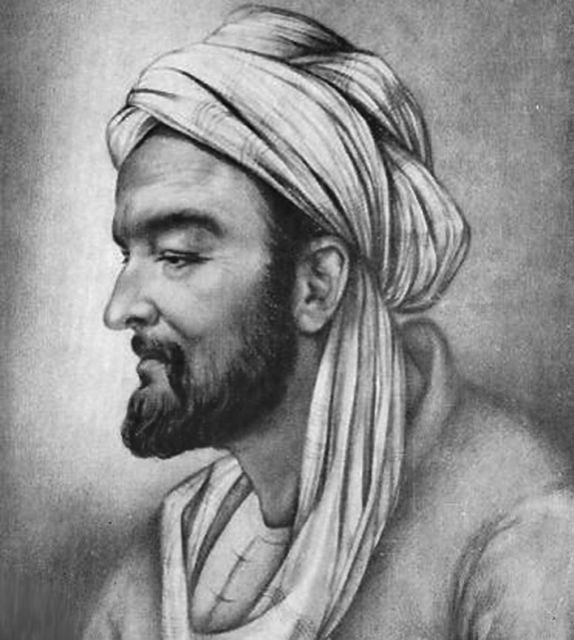
\includegraphics[width=5cm]{images/abu_ali.jpg}
  \caption*{«Коль смолоду избрал к заветной правде путь, \\
 С невеждами не спорь, советы их забудь». }
 \end{center}
\end{figure}


Каждый Мудрец может постигнуть Истину самостоятельно с вероятностью $1/9$ или же от соседа\footnote{Студенты постигают Истину примерно также!}. Независимо от способа постижения Истины, просветлённый Мудрец поделится Истиной с соседом слева с вероятностью $2/9$ и с соседом справа также с вероятностью $2/9$ (независимо от соседа слева).


\begin{enumerate}
\item Какова вероятность того, что Абу Али Хусейн ибн Абдуллах ибн аль-Хасан ибн Али ибн Сина постигнет Истину?
\item Как изменится ответ, если ряд Мудрецов бесконечен в обе стороны?
\end{enumerate}

\end{enumerate}

\subsection{Кр 1 ИП, 27.10.2016, решения}

\begin{enumerate}
\item
\begin{enumerate}
\item Для удобства занумеруем макаронины и выделим у каждой левый и правый конец. Взяли правый конец первой макаронины и подвязали случайной. Взяли свободный конец только что подвязанной макаронины и подвязали случайно. И так далее.
\[
\frac{2n-2}{2n-1}\cdot \frac{2n-4}{2n-3}\cdot \ldots \cdot \frac{2}{3} \cdot 1
\]
\item Допустим, что при $n$ макаронинах в среднем образуется $e_n$ колец. После первого соединения задача сводится к меньшему числу макаронин, важно только учесть, образовалось ли кольцо при первом соединении:
\[
e_n = e_{n-1} + 1/(2n-1) \cdot 1
\]
\item Количество коротких колец можно разбить в сумму, $X=Z_1 + \ldots + Z_n$. Вероятность завязывания конкретной макаронины в кольцо равна $1/(2n-1)$: «левый конец» надо привазять именно к «правому». Значит, $\E(X)=n/(2n-1)$.
\end{enumerate}

\item
\begin{enumerate}
\item Рассмотрим обратную ситуацию: на планете есть точка, из которой связаться хотя бы с одним пепелацем нельзя. Такое возможно, если все, кроме одного, сели в одну полуокружность.
\[
\P(\text{есть точка без связи}) = n \cdot \left(\frac{1}{2}\right)^{n-1} \Rightarrow \P(\text{из любой точки есть связь}) = 1 - n \cdot \left(\frac{1}{2}\right)^{n-1}
\]
\item Зафиксируем координату посадки первого пепелаца и возьмём её за точку отсчёта. Изобразим на плоскости возможные значения центральных углов между первым пепелацем и оставшимися и закрасим нужные участки. Получим 3/8.
\item Зафиксируем координату посадки первого пепелаца. Обозначим центральный угол между первым и вторым пепелацами $\alpha$. Функция плотности имеет вид: $p(\alpha) = \frac{\sin(\alpha)}{2}$

Итог: $\int_0^{\pi/2} p(\alpha) \frac{\alpha + \pi}{2\pi} d \alpha + \int_{\pi/2}^{\pi}  p(\alpha) \frac{\pi - \alpha}{2\pi} d \alpha = \frac{\pi + 2}{4\pi}$
\end{enumerate}

\item Вспомним для начала, что площадь круга равна $\pi r^2$, а площадь сферы равна $4\pi r^2$. Составим из маленьких треугольничков многогранник очень похожий на сферу с единичным радиусом. Площадь этого многогранника будет примерно равна $4\pi$. Проекция многогранника представляет собой примерно круг единичного радиуса. Проекция имеет два слоя. С учётом обоих слоёв площадь проекции равна $2\pi$. Значит отношение площади проекции к площади многогранника равно $1/2$.

От взаимного расположения треугольничков в пространстве ожидаемая площадь проекции не зависит в силу аддитивности математического ожидания.

Ответ: 21 см$^2$.

\item
\begin{enumerate}
\item Мысленно отметим на окружности три точки: места ударов Брюса Ли и точку, где схватился Чак Норрис. Можно считать, что эти три точки равномерно и независимо распределены по окружности. Следовательно, среднее расстояние между соседними точками равно $1/3$. Чак Норрис берёт два кусочка, слева и справа от своей точки. Значит ему в среднем достаётся $2/3$ окружности.
\item Объявим точку, где схватился Чак Норрис нулём. Координаты двух ударов изобразим на плоскости. Закрашиваем подходящий участок. Вероятность того, что кусок Брюса Ли длиннее, равна $1/4$.
\end{enumerate}

\item  Рассмотрим совершенно конкурентный невольничий рынок начинающих певиц. Певицы в хорошем настроении продаются по $V_1$, в депрессии — по $V_2$. Получаем систему уравнений:
\[
\begin{cases}
  V_1 = 0.75 + (0.5 V_1 + 0.5 V_2) \\
  V_2 = \max_x \sqrt{x}V_1 + (1 - \sqrt{x})V_2 - x
\end{cases}
\]
Оптимизируем и получаем, $x^* = (V_1 - V_2)^2/4$. Из первого уравнения находим $(V_1 - V_2)/2=0.75$.

\item Да. Например, такая. До общения с Джульеттой подкидывать монетку до выпадения первого орла и запомнить число потребовавшихся подбрасываний. Пусть это будет число $X$. Открыть равновероятно левую или правую руку Джульетты. Если открытое число больше $X$, то сказать, что оно большее, иначе сказать, что меньшее.
\item Если $\gamma$ — вероятность самостоятельного познания Истины, а $\alpha$ — передачи Истины отдельно в каждую из сторон, то
\[
p = \gamma + (1-\gamma) p \alpha.
\]

То есть $p=\gamma/(1-\alpha(1-\gamma))$.

Для решения второго пункта наложим на Абу Али Хусейн ибн Абдуллах ибн аль-Хасан ибн Али ибн Сина обет молчания. Это не повлияет на вероятность постижения им Истины, однако превратит задачу в две уже решённых :) Получаем
\[
q = \gamma + (1-\gamma)(2p\alpha - p^2\alpha^2)
\]
\end{enumerate}


\subsection{Кр 2 базовый поток, 09-12-2016}


\textbf{Неравенства Берри–Эссеена:} Для любых $n \in \mathbb{N}$ и всех $x \in \mathbb{R}$ имеет место оценка:
\[
    \bigl|F_{S_n^{*}}(x) - \Phi(x)\bigr| \leq 0.48 \cdot \frac{\E(|\xi_i - \E\xi_i|^3)}{\Var^{3/2}(\xi_i)\cdot\sqrt{n}} \text{,}
\]
где $\Phi(x) = \int_{-\infty}^{x}\frac{1}{\sqrt{2\pi}}e^{-\frac{t^2}{2}}\,dt$, \; $S_n^* = \frac{S_n - \E(S_n)}{\sqrt{\Var(S_n)}}$, \; $S_n = \xi_1 + \ldots + \xi_n$

\textbf{Распределение Пуассона:} Случайная величина $\xi$ имеет распределение Пуассона с параметром $\lambda > 0$,  если она принимает целые неотрицательные значения с вероятностями $\P(\{\xi = k\}) = \frac{\lambda^k}{k!}e^{-\lambda}$. Приличным студентам должно быть известно, что в этом случае $\E(\xi) = \Var(\xi) = \lambda$.

\begin{enumerate}
\item Пусть $\E(\xi) = 1$, $\E(\eta) = -2$, $\Var(\xi) = 1$, $\E(\eta^2) = 8$, $\E(\xi \eta) = -1$. Найдите
\begin{enumerate}
\item $\E(2\xi-\eta+1)$, $\Cov(\xi, \,\eta)$, $\Corr(\xi, \,\eta)$,  $\Var(2\xi-\eta+1)$;
\item $\Cov(\xi+\eta, \,\xi+1)$, $\Corr(\xi+\eta, \,\xi+1)$, $\Corr(\xi+\eta-24, \,365 - \xi - \eta)$, $\Cov(2016\cdot\xi, \, 2017)$.
\end{enumerate}

\item
Совместное распределение доходностей акций двух компаний задано с помощью таблицы:

\begin{center}
\begin{tabular}{ccc}
\toprule
         & $\eta=-1$ & $\eta=1$ \\
\midrule
$\xi=-1$  & $0.1$       & $0.2$   \\
$\xi=0$   & $0.2$       & $0.2$   \\
$\xi=2$   & $0.2$       & $0.1$   \\
\bottomrule
\end{tabular}
\end{center}

\begin{enumerate}
  \item Найдите частные распределения случайных величин $\xi$ и $\eta$.
  \item Найдите $\Cov(\xi,\,\eta)$.
  \item Сформулируйте определение независимости дискретных случайных величин.
  \item Являются ли случайные величины $\xi$ и $\eta$ независимыми?
  \item Найдите условное распределение случайной величины $\xi$, если $\eta = 1$.
  \item Найдите условное математическое ожидание случайной величины $\xi$, если $\eta = 1$.
  \item Найдите математическое ожидание и дисперсию величины $\pi = 0.5\, \xi + 0.5\, \eta$.
  \item Рассмотрим портфель, в котором $\alpha$ — доля акций с доходностью $\xi$ и $(1 - \alpha)$ — доля акций с доходностью $\eta$. Доходность этого портфеля есть случайная величина
  \[\pi(\alpha) = \alpha \xi + (1-\alpha)\eta.\]
  Найдите такую долю $\alpha \in [0;\,1]$, при которой доходность портфеля $\pi(\alpha)$ имеет наименьшую дисперсию.
\end{enumerate}

\item Число посетителей сайта \url{pokrovka11.wordpress.com} за один день имеет распределение Пуассона с математическим ожиданием 250.
\begin{enumerate}
  \item Сформулируйте неравенство Маркова. При помощи данного неравенства оцените вероятность того, что за один день сайт посетят более 500 человек.
  \item Сформулируйте неравенство Чебышева. Используя данное неравенство, определите наименьшее число дней, при котором с вероятностью не менее 99\% среднее за день число посетителей будет отличаться от 250 не~более чем на 10.
  \item Решите предыдущий пункт с помощью центральной предельной теоремы.
  \item Сформулируйте закон больших чисел. Обозначим через $\xi_i$ число посетителей сайта за $i$-ый день. Найдите предел по вероятности последовательности $\frac{\xi_1^2 + \ldots + \xi_n^2}{n}$ при $n \rightarrow \infty$.
\end{enumerate}

\item Отведав медовухи, Винни–Пух совершает случайное блуждание на прямой. Он стартует из начала координат и в каждую следующую минуту равновероятно совершает шаг единичной длины налево или направо. Передвижения Винни-Пуха схематично изображены на следующем рисунке.
\begin{figure}[h]
    \noindent\centering{
    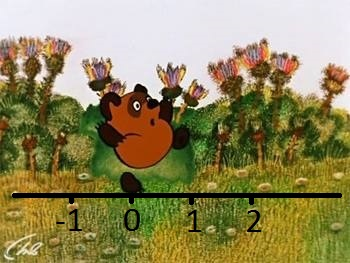
\includegraphics[width=80mm]{images/Winnie_the_Pooh_and_Medovuh.jpg}
    }
    \caption{Случайные бродилки.}
    \label{wun762hkej}
\end{figure}
\begin{enumerate}
  \item Сформулируйте центральную предельную теорему.
  \item При помощи центральной предельной теоремы оцените вероятность того, что ровно через час блужданий Винни-Пух окажется в области $(-\infty; \, -5]$.
  \item Используя неравенство Берри–Эссеена оцените погрешность вычислений предыдущего пункта.
\end{enumerate}


\item
Cлучайные величины $\xi$ и $\eta$ означают время безотказной работы рулевого управления и двигателя автомобиля соответственно. Время измеряется в годах. Совместная плотность имеет вид:
\[
f_{\xi, \,\eta}(x,\,y) =
\begin{cases}
0.005\,e^{-0.05\,x-0.1\,y} & \text{ при } x > 0, y > 0, \\
0                    & \text{ иначе.}
\end{cases}
\]

\begin{enumerate}
  \item Найдите частные плотности распределения случайных величин $\xi$ и $\eta$.
  \item Являются ли случайные величины $\xi$ и $\eta$ независимыми?
  \item Найдите вероятность того, что двигатель прослужит без сбоев более пяти лет.
  \item Найдите вероятность того, что двигатель прослужит без сбоев более восьми лет, если он уже проработал без сбоев три года.
  \item Найдите условное математическое ожидание безотказной работы рулевого управления, если двигатель проработал без сбоев пять лет,  $\E(\xi | \eta = 5)$.
  \item Найдите вероятность того, что рулевое управление проработает без сбоев на два года больше двигателя,  $\P(\{\xi - \eta > 2\})$.
\end{enumerate}

\item Бонусная задача

Случайная величина $\xi$ имеет плотность распределения
\[
    f_{\xi}(x) = \frac{1}{2} \cdot \frac{1}{\sqrt{2\pi}}e^{-\frac{(x-1)^2}{2}} + \frac{1}{2} \cdot \frac{1}{\sqrt{2\pi}}e^{-\frac{(x+1)^2}{2}} \text{.}
\]

\begin{enumerate}
\item Найдите $\E(\xi)$, $\E(\xi^2)$, $\Var(\xi)$.
\item Покажите, что функция $f_{\xi}(x)$, действительно, является плотностью распределения.
\end{enumerate}


\end{enumerate}



\subsection{Кр 2 базовый поток, 09-12-2016, решения}

\begin{enumerate}
\item \begin{enumerate}
\item $\E (2\xi - \eta +1) = 2 \E (\xi) - \E (\eta) + 1 = 2\cdot 1 - (-2) + 1 = 5 $

$\Cov (\xi, \eta) = \E (\xi \eta) - \E(\xi) \E(\eta) = -1 - \cdot 1 \cdot (-2) = 1$

$\Corr (\xi, \eta) = \frac{\Cov(\xi, \eta)}{\sqrt[]{\Var(X) \cdot \Var(Y)}} = \frac{1}{\sqrt{1 \cdot (8-(-2)^2)}} = \frac{1}{2}$

$\Var (2\xi - \eta + 1) = 4\Var(\xi) + \Var(\eta) - 2 \Cov (2\xi, \eta) = 4 \cdot 1 + 4 - 4 \cdot 1 = 4$

\item $\Cov(\xi + \eta, \xi + 1) = \Cov(\xi) + \Cov(\xi, 1) + \Cov(\eta, \xi) + \Cov(\eta, 1) = 1 +1 = 2$

$\Corr(\xi + \eta , \xi + 1) = \frac{\Cov(\xi + \eta , \xi + 1)}{\sqrt{\Var(\xi + \eta)\cdot \Var (\xi + 1)}} = \frac{2}{\sqrt{(1+4+2\cdot 1) \cdot 1}} = \frac{2}{\sqrt{7}}$

$\Corr(\xi + \eta - 24, 365 - \xi - \eta) = -1$

$\Cov(2016\cdot \xi, 2017) = 0$

\end{enumerate}
\item \begin{enumerate}
\item \begin{tabular}{cccc}
\toprule
$\xi$ & $-1$ & $0$ & $2$ \\ \midrule
$\P(\cdot)$ & $0.3$ & $0.4$ & $0.3$ \\ \bottomrule
\end{tabular}
\hspace{1cm}
\begin{tabular}{ccc}
\toprule
$\eta$ & $-1$ & $1$ \\ \midrule
$\P(\cdot)$ & $0.5$ & $0.5$ \\ \bottomrule
\end{tabular}

$\E(\xi) = -1 \cdot 0.3 + 0 \cdot 0.4 + 2 \cdot 0.3 = 0.3$

$\E (\xi^2) = (-1)^2 \cdot 0.3 + 0^2 \cdot 0.4 + 2^2 \cdot 0.3 = 1.5$

$\Var(\xi) = \E(\xi^2) - (\E(\xi))^2 = 1.5 - 0.3^2 = 1.41$

$\E(\eta) = -1 \cdot 0.5 + 1 \cdot 0.5 = 0$

$\E(\eta^2) = (-1)^2 \cdot 0.5 + 1^2 \cdot 0.5 = 1$

$\Var(\eta) = \E(\eta^2)-(\E(\eta))^2 = 1 - 0^2 = 1$

\item \begin{tabular}{cccccc}
\toprule
$\xi \cdot \eta$ & $-2$ & $-1$ & $0$ & $1$ & $2$ \\ \midrule
$\P(\cdot)$ & $0.2$ & $0.2$ & $0.4$ & $0.1$ & $0.1$ \\ \bottomrule
\end{tabular}

$\E(\xi\cdot\eta) = (-2) \cdot 0.2 + (-1) \cdot 0.2 + 0 \cdot 0.4 + 1\cdot 0.1 + 2 \cdot 0.1 = -0.3$

$\Cov(\xi, \eta) = \E(\xi\cdot\eta) - \E(\xi)\cdot\E(\eta) = -0.3 - 0.3 \cdot 0 = -0.3$
\item Пусть случайная величина $X$ принимает значения $a_1, \ldots, a_m$, случайная веилчина $Y$ принимает значения $b_1, \ldots, b_n$. Тогда случйаня величина $X$ и $Y$ называются независимыми, если $\forall i=1, \ldots, m \quad \forall j=1, \ldots, n: \P(X = a_i \cap Y = b_j) = P(X = a_i) \cdot P(Y = b_j)$
\item Заметим, что $\P (\xi = -1 \cap \eta=-1)=0.1$, $\P(\xi=-1)=0.3$ и $\P(\eta=-1)=0.5$.

Тогда поскольку $\P (\xi = -1 \cap \eta=-1) \neq \P(\xi=-1) \cdot \P(\eta=-1)$, случайные величины $\xi$ и $\eta$ не являются независимыми.
\item $\P (\xi = -1 \cap \eta=1) = \frac{\P (\xi = -1 \cap \eta=1)}{\P(\eta=1)} = \frac{0.2}{0.5} = \frac{2}{5}$

$\P (\xi = 0 \cap \eta=1) = \frac{\P (\xi = 0 \cap \eta=1)}{\P(\eta=1)} = \frac{0.2}{0.5} = \frac{2}{5}$

$\P (\xi = 2 \cap \eta=1) = \frac{\P (\xi = 2 \cap \eta=1)}{\P(\eta=1)} = \frac{0.1}{0.5} = \frac{1}{5}$

Следовательно, условное распределение случайной величины $\xi$ при условии $\{\eta=1\}$ может быть описано следующей таблицей:

\begin{tabular}{cccc}
\toprule
$\xi$ & $-1$ & $0$ & $2$ \\ \midrule
$\P(\cdot)$ & $2/5$ & $2/5$ & $1/5$ \\ \bottomrule
\end{tabular}
\item $\E(\xi \mid \eta = 1) = -1 \cdot \frac{2}{5} + 0 \cdot \frac{2}{5} + 2 \cdot \frac{1}{5} = 0$
\item $\E(\pi) = \E(0.5 \xi + 0.5 \eta) = 0.5 \E(\xi) + 0.5 \E(\eta) = 0.15$

\begin{multline*}
\Var(\pi) = \Var(0.5 \xi + 0.5 \eta) = \Var(0.5 \xi) + \Var(0.5\eta) + 2 \Cov (0.5\xi, 0.5\eta) = \\
= 0.25\Var(\xi) + 0.25\Var(\eta) + 2 \cdot 0.5 \cdot 0.5 \Cov(\xi, \eta) = \\
= 0.25 \cdot 1.41 + 0.25 \cdot 1 + 2 \cdot 0.5 \cdot 0.5 \cdot (-0.3) = 0.4525
\end{multline*}
\item
\begin{multline*}
\Var(\pi(\alpha)) = \Var(\alpha \xi + (1-\alpha)\eta) = \alpha^2\Var(\xi) + (1-\alpha)^2 \Var(\eta) + \\
+ 2\alpha(1-\alpha) \Cov(\xi, \eta) = 1.41 \cdot \alpha^2 + 1\cdot (1-\alpha)^2 + 2\alpha(1-\alpha) \cdot (-0.3) = \\
= 1.41 \cdot \alpha^2 + (1-\alpha)^2 - 0.6 \cdot (\alpha - \alpha^2) \to \min_\alpha
\end{multline*}
\begin{multline*}
\frac{\partial}{\partial \alpha} \Var(\pi(\alpha)) = 2 \cdot 1.41 \cdot \alpha -2(1-\alpha) -0.6\cdot(1-2\alpha) = \\
= 2.82 \cdot \alpha - 2 + 2\alpha - 0.6 + 1.2 \cdot \alpha = 6.02 \cdot \alpha - 2.6 = 0
\end{multline*}
\[
\alpha = \frac{2.6}{6.02} = 0.4319
\]
\end{enumerate}
\item \begin{enumerate}
\item Для любой неотрицательной случайной величины $X$ и любого числа $\lambda > 0$ справедлива оценка: $\P(X>\lambda) \leq \frac{\E(X)}{\lambda}$

Пусть случайная величина $\xi_i$ означает число посетителей сайта за $i$-ый день. По условию, $\xi_i \sim Pois(\lambda=250)$. Известно, что если $\xi \sim Pois(\lambda)$, то $\E(\xi) = \Var(\xi) = \lambda$.

Имеем:
\[
\P(\xi_i >500) \leq \P(\xi_i \geq 500) \leq \frac{\E(\xi_i)}{500} = \frac{250}{500} = \frac{1}{2}
\]
\item Для любой случайной величины $X$ с конечным $\E(X)$ и любого положительного числа $\epsilon > 0$ имеет место неравенство: $\P(X-\E(X)\geq\epsilon)\leq\frac{\Var(X)}{\epsilon^2}$

Обозначим $\bar{\xi}_n := \frac{1}{n} \left(\xi_1 + \ldots + \xi_n\right)$ – среднее число посетителей сайта за $n$ дней. Тогда
\[
\E(\bar{\xi}_n) = \E\left(\frac{1}{n} \sum_{i=1}^{n} \xi_i\right) = \frac{1}{n} \sum_{i=1}^{n} \E(\xi_i) = \frac{1}{n} \cdot n \cdot \lambda = \lambda = 250
\]
\[
\Var(\bar{\xi}_n) = \Var\left(\frac{1}{n} \sum_{i=1}^{n} \xi_i\right) = \frac{1}{n^2} \sum_{i=1}^{n} \Var (\xi_i) = \frac{n \cdot \lambda}{n^2} = \frac{\lambda}{n} = \frac{250}{n}
\]
Оценим вероятность
\[
\P(\vert\bar{\xi}_n-250\vert > 10) \leq \frac{\Var(\bar{\xi}_n)}{100} = \frac{250}{100\cdot n}
\]
Следовательно, $1 - \frac{250}{100\cdot n} \leq \P(\vert\bar{\xi}_n-250\vert > 10)$.

Найдём наименьшее целое $n$, при котором $0.99 \leq 1 - \frac{250}{100\cdot n}$.

Имеем:
\[
0.99 \leq 1 - \frac{250}{100\cdot n} \Leftrightarrow \frac{250}{100\cdot n} \Leftrightarrow n \geq \frac{250}{100 \cdot 0.01} \Leftrightarrow n  \geq 250
\]
Стало быть, $n=250$ – наименьшее число дней, при котором с вероятностью не менее $99\%$ среднее число поситителей будет отличаться от $250$ не более чем на $10$.
\item  Требуется найти наименьшее целое $n$, при котором $\P(\vert\bar{\xi}_n-250\vert \leq 10)=0.99$

Имеем:
\begin{multline*}
\P(\vert\bar{\xi}_n-250\vert \leq 10)=0.99 \Leftrightarrow \P(-10\leq \bar{\xi}_n -250 \leq 10) =0.99 \Leftrightarrow \\
\Leftrightarrow  \P(-10n \leq S_n-250 \leq 10n) =0.99
\end{multline*}
\[
\E(S_n) = \E(\xi_1 + \ldots + \xi_n) = \E(\xi_1) + \ldots + \E(\xi_n) = 250\cdot n
\]
\[
\Var(S_n) = \Var(\xi_1 + \ldots + \xi_n) = \Var(\xi_1) + \ldots + \Var(\xi_n) = 250 \cdot n
\]
\begin{multline*}
\P\left(\frac{-10n}{\sqrt{250n}} \leq \frac{S_n - \E (S_n)}{\sqrt{\Var(S_n)}} \leq \frac{10n}{\sqrt{250n}}\right) =0.99 \Leftrightarrow 2 \Phi \left(\frac{10n}{\sqrt{250n}}\right) -1 = 0.99 \\
\Phi \left(\frac{10n}{\sqrt{250n}}\right) = \frac{1 + 0.99}{2} \Leftrightarrow \frac{10n}{\sqrt{250n}} = 2.58 \Leftrightarrow \sqrt{n} = 2.58 \cdot \frac{\sqrt{250}}{10} \Leftrightarrow n = 16.641
\end{multline*}
Следовательно, наименьшее целое $n$, есть $n=17$.
\item Пусть $X_1, X_2, \ldots, X_n, \ldots$ – последовательность независимых случайных величин с одинаковыми конечными математическими ожиданимяи и фиксированными конечными дисперсиями. Тогда $\frac{X_1 + \ldots + X_n}{n} \stackrel{\P}{\to} \E(X_i)$ при $n \to \infty$.

В нашем случае случаные величины $\xi_1^2, \xi_2^2, \ldots, \xi_n^2, \ldots$ – независимы,

$\E(\xi_1^2) = \ldots = \E(\xi_n^2) = \ldots < + \infty$ и $\Var(\xi_1^2) = \ldots = \Var(\xi_n^2) = \ldots < + \infty$ . Поэтому в соответствии с ЗБЧ имеем:
\[
\frac{\xi_1^2 +\ldots+ \xi_n^2}{n} \stackrel{\P}{\to} \E(\xi_i^2) = \Var(\xi_i) +\E(\xi_i)^2 = \lambda + \lambda^2 = \lambda(\lambda+1) = 250\cdot251 = 62700
\]
\end{enumerate}

\item \begin{enumerate}
\item Пусть $X_1, X_2, \ldots, X_n, \ldots$ – последовательность независимых, одинаково распределённых случайных величин с $0<\Var(X_i)<\infty$, $i \in \mathbb{N}$.  Тогда для любого (борелевского) множества $B \subseteq R$ имеет место $\lim_{n \to \infty} \P\left(\frac{S_n - \E(S_n)}{\sqrt{\Var(S_n)}} \in B\right) = \int_B \frac{1}{\sqrt{2\pi}}e^{-t^2/2} dt$, где $S_n := X_1, \ldots, X_n$, $n \in \mathbb{N}$.
\item Введём случайную величину
\[
X_i = \begin{cases}
1, & \text{если на i-ом шаге Винни-Пух пошёл направо} \\
0, & \text{если пошёл налево}
\end{cases}
\quad i=1,\ldots, n;
\]
Тогда $S_n := X_1 +\ldots+X_n$ означает местоположение Винни-Пуха в $n$-ую минуту его блужданий по прямой.

$\E(X_i) = -1 \cdot 1/2 + 1 \cdot 1/2 = 0$,

$\E(X_i^2) = (-1)^2 \cdot 1/2 + (1)^2 \cdot 1/2 = 1$,

$\Var(X_i) = \E(X_i^2) - \E(X_i)^2 = 1$,

$\E(S_n) = \E(X_1 + \ldots + X_n ) = \E(X_1) + \ldots + \E(X_n) = 0$,

$\Var(S_n) = \Var(X_1 + \ldots + X_n ) = \Var(X_1) + \ldots + \Var(X_n) = n$

\begin{multline*}
\P(S_n \in (-\infty, -5]) = \P(S_n \leq -5) = \P\left( \frac{S_n-\E(S_n)}{\sqrt{\Var(S_n)}} \leq \frac{-5-0}{\sqrt{n}} \right) \stackrel{n=60}{=} \\
=\P\left( \frac{S_n-\E(S_n)}{\sqrt{\Var(S_n)}} \leq -0.6454\right) \approx \int_{-\infty}^{-0.6454} \frac{1}{\sqrt{2\pi}} e^{-t^2/2} dt = \\
= \Phi(-0.6454) = 1-\Phi(0.6454) \approx0.2593
\end{multline*}
\item Для любых $n \in \mathbb{N}$ и всех $x \in \mathbb{R}$ имеет место оценка:
\[
\bigl|F_{S_n^{*}}(x) - \Phi(x)\bigr| \leq 0.48 \cdot \frac{\E(|\xi_i - \E\xi_i|^3)}{\Var^{3/2}(\xi_i)\cdot\sqrt{n}} \text{,}
\]
где $\Phi(x) = \int_{-\infty}^{x}\frac{1}{\sqrt{2\pi}}e^{-\frac{t^2}{2}}\,dt$, \; $S_n^* = \frac{S_n - \E(S_n)}{\sqrt{\Var(S_n)}}$, \; $S_n = \xi_1 + \ldots + \xi_n$

В нашем случае:
\[
\P\left( \frac{S_{60} - \E(S_{60})}{\sqrt{\Var(S_{60})}} \leq -0.6454 \right) = \P(S^*_{60} \leq -0.6454) =
F_{S^*_{60}} (-0.6454)
\]
Согласно неравенству Берри-Эссеена, погрешность $\vert F_{S^*_{60}} (-0.6454) - \Phi(-0.6454) \vert$ оценивается сверху величиной
\[
0.48 \cdot \frac{\E(\vert X_i - \E(X_i) \vert^3 )}{\Var(X_i)^{3/2} \cdot \sqrt{n}} = 0.48 \cdot \frac{\E(\vert X_i \vert^3)}{1\cdot\sqrt{60}} = \frac{0.48}{\sqrt{60}} \approx0.062
\]
\end{enumerate}
\item \begin{enumerate}
\item Сначала найдём плотность распределения случайной величины $X$. Пусть $x \leq 0 $, тогда $f_X (X) = \int_{-\infty}^{+\infty} f_{X, Y} (x, y) dy  = 0$;

Пусть $x >0 $, тогда
\begin{multline*}
f_X (X) = \int_{-\infty}^{+\infty} f_{X, Y} (x, y) dy = \int_{0}^{+\infty} 0.005 e^{-0.05x-0.1y} dy = \\
= 0.005e^{-0.05x} \int_{0}^{+\infty} e^{-0.1y} dy = 0.005e^{-0.05x} \cdot \left(-10e^{-0.1y} \right) \bigg\vert_{y=0}^{y=+\infty} = 0.05 e^{-0.05x}
\end{multline*}
Таким образом, имеем:
\[
f_X (x) = \begin{cases}
0.05 e^{-0.05x} & \text{при } x>0 \\
0 & \text{при } x \leq 0
\end{cases}
\]
То есть $X \sim Exp(\lambda=0.05)$ – случайная величина $X$ имеет показательное распределение с параметром $\lambda = 0.05$.

Теперь найдём плотность распределения случайной величины $Y$.

Пусть $y \leq 0 $, тогда $f_Y (y) = \int_{-\infty}^{+\infty} f_{X, Y} (x, y) dx  = 0$.

Пусть $y > 0 $, тогда
\begin{multline*}
f_Y (y) = \int_{-\infty}^{+\infty} f_{X, Y} (x, y) dx  = \int_{0}^{+\infty} 0.005 e^{-0.05x-0.1y} dx = \\
= 0.005e^{-0.1y} \int_{0}^{+\infty} e^{-0.05x} dx = 0.005e^{-0.1y} \cdot \left(-20e^{-0.05x} \right) \bigg\vert_{x=0}^{x=+\infty} = 0.1 e^{-0.1y}
\end{multline*}
Таким образом, имеем:
\[
f_Y (y) = \begin{cases}
0.1 e^{-0.1y} & \text{при } y>0 \\
0 & \text{при } y \leq 0
\end{cases}
\]
То есть $Y \sim Exp(\lambda=0.1)$ – случайная величина $Y$ имеет показательное распределение с параметром $\lambda = 0.1$.
\item Поскольку для любых точек $x, y \in \mathbb{R}$ справедливо равенство $f_{X, Y} (x, y) = f_X (x) \cdot f_Y (y)$, случайные величины $X$ и $Y$ являются независимыми.
\item Найдём вероятность $\P(Y>5)$:
\[
\P(Y>5) = \int_{5}^{+\infty} f_Y (y) dy = \int_{5}^{+\infty}  0.1 e^{-0.1y} dy = 0.1 \cdot (-10 e^{-0.1x}) \bigg\vert_{y=5}^{y=+\infty} = e^{-0.5} \approx0.6065
\]
\item Требуется найти условную вероятность $\P(Y>8 \mid Y \geq 3)$. Для этого предварительно найдём вероятности $\P(Y>8)$ и $\P(y \geq 3)$:
\[
\P(Y>8) = \int_{8}^{+\infty} f_Y (y) dy  = \int_{8}^{+\infty}  0.1 e^{-0.1y} dy = 0.1 \cdot (-10 e^{-0.1x}) \bigg\vert_{y=8}^{y=+\infty} = e^{-0.8}
\]
\[
\P(Y \geq 3) =  \int_{3}^{+\infty} f_Y (y) dy   =  \int_{3}^{+\infty}  0.1 e^{-0.1y} dy = 0.1 \cdot (-10 e^{-0.1x}) \bigg\vert_{y=3}^{y=+\infty} = e^{-0.3}
\]
Теперь находим требуемую условную веростность:
\[
\P(Y>8 \mid Y \geq 3) = \frac{\P((Y > 8) \cap
(Y \geq 3))}{\P(Y \geq 3)} = \frac{\P(Y>8)}{\P(Y \geq 3) } = \frac{e^{-0.8}}{e^{-0.3}} = e^{-0.5} \approx0.6065
\]
\item Сначала найдём условную плотность распределения случайной величины $X$ при условии $Y=y$:
\begin{multline*}
f_{X \mid Y} (x \mid y) = \begin{cases}
\frac{f_{X \mid Y} (x, y)}{f_Y (y)} & \text{при } f_Y (y) 0 \\
0 & \text{иначе}
\end{cases} =
\begin{cases}
\frac{0.005e^{-0.05x-0.1y}}{0.1e^{-0.1y}} & \text{при } x>0, \quad y>0 \\
0 & \text{иначе}
\end{cases} = \\
= \begin{cases}
0.05 e^{-0.05x} & \text{при } x>0, \quad y>0 \\
0 & \text{иначе}
\end{cases} =
\begin{cases}
f_X (x) & \text{при } y > 0 \\
0 & \text{при } y \leq 0
\end{cases}
\end{multline*}
Теперь находим условное математическое ожидание
\[
\E(X \mid Y=5) = \int_{-\infty}^{+\infty} xf_{X\mid Y} (x \mid 5) dx =  \int_{-\infty}^{+\infty} xf_{X} (x) dx = \E(X) = \frac{1}{0.05} =20
\]
Здесь мы воспользовались известным фактом, что если $X\sim Exp(\lambda)$, то $\E(X) = \frac{1}{\lambda}$
\item Требуется найти вероятность $\P(X-Y > 2)$. Для этого введём множества

$B:=\{(x, y) \in \mathbb{R} : y < x-2 \}$ и $C := \{ (x,y) \in \mathbb{R} : y < x-2, x>0, y> 0  \}$.

Заметим, что искомая вероятность  $\P(X-Y > 2)$ может быть записана в виде
\[
\P(X-Y > 2) = \P((X, Y) \in B ) = \int \int_B f_{X, Y} (x, y) dx dy = \int \int_C f_{X, Y} (x, y) dx dy
\]
Стало быть, искомая вероятность
\begin{multline*}
\P(X-Y > 2) = \int \int_C f_{X, Y} (x, y) dx dy = \int_{2}^{+\infty} \left[ \int_{0}^{x-2} f_{X, Y} (x, y) dy \right] dx =\\
= \int_{2}^{+\infty} \left[ \int_{0}^{x-2} 0.005e^{-0.05x-0.1y}dy \right] dx
= \int_{2}^{+\infty} \left[ 0.005e^{-0.05x} \cdot (-10e^{-0.1y}) \bigg\vert_{y=0}^{y=x-2} \right] dx = \\
=  \int_{2}^{+\infty} \left[ 0.005e^{-0.05x} \cdot\left(1-e^{-0.1(x-2)}  \right) \right] dx  = \int_{2}^{+\infty} 0.005e^{-0.05x} dx - \\
- \int_{2}^{+\infty} 0.005e^{-0.05x-0.1x+0.2} dx
= 0.05 \cdot \left( -\frac{1}{0.05}e^{-0.05x}  \right) \bigg\vert_{x=2}^{x=+\infty} - \\
- e^{0.02} \cdot 0.05 \cdot \left( \frac{1}{0.15} e^{-0.15x} \right) \bigg\vert_{x=2}^{x=+\infty}
= e^{-0.1} -\frac{1}{3} e^{-0.1} = \frac{2}{3}e^{-0.1}  \approx 0.6032
\end{multline*}
\end{enumerate}
\item Для решения задачи воспользуемся хорошо известными соотношениями:
\[
\int_{-\infty}^{+\infty} \frac{1}{\sqrt{2\pi\sigma^2}} e^{-\frac{(x-\mu)^2}{2\sigma^2}} dx = 1
\]
\[
\int_{-\infty}^{+\infty} x\frac{1}{\sqrt{2\pi\sigma^2}} e^{-\frac{(x-\mu)^2}{2\sigma^2}} dx = \mu
\]
\[
\int_{-\infty}^{+\infty} x^2 \frac{1}{\sqrt{2\pi\sigma^2}} e^{-\frac{(x-\mu)^2}{2\sigma^2}} dx = \mu^2 + \sigma^2
\]
\begin{enumerate}
\item Указанная в задании функция $f_X$ является плотностью распределения, так как она удовлетворяет двум условиям:  $f_X$ является неотрицательной и интеграл от функции $f_X$ в пределах от  $-\infty$ до $+\infty$ равен единице:
\[
\int_{-\infty}^{+\infty} f_X (x) dx = \frac{1}{2} \cdot \int_{-\infty}^{+\infty}  \frac{1}{\sqrt{2\pi}} e^{-\frac{(x-1)^2}{2\sigma^2}} dx  + \frac{1}{2} \int_{-\infty}^{+\infty} \cdot \frac{1}{\sqrt{2\pi}} e^{-\frac{(x+1)^2}{2}} dx = 1
\]
\item $\E(X) =\int_{-\infty}^{+\infty} xf_X (x) dx =  \frac{1}{2} \cdot \int_{-\infty}^{+\infty} x \frac{1}{\sqrt{2\pi}} e^{-\frac{(x-1)^2}{2\sigma^2}} dx  + \frac{1}{2}\int_{-\infty}^{+\infty} \cdot x \frac{1}{\sqrt{2\pi}} e^{-\frac{(x+1)^2}{2}} dx = 1- 1=  0$
\item  \begin{multline*}
\E(X^2) = \int_{-\infty}^{+\infty} x^2 f_X (x) dx  =  \frac{1}{2} \cdot \int_{-\infty}^{+\infty} x^2 \frac{1}{\sqrt{2\pi}} e^{-\frac{(x-1)^2}{2\sigma^2}} dx  + \frac{1}{2} \int_{-\infty}^{+\infty}\cdot x^2 \frac{1}{\sqrt{2\pi}} e^{-\frac{(x+1)^2}{2}} dx = \\
= 1^2 + 1^2 + (-1)^2 + 1^2 =  2
\end{multline*}
\item $\Var(X) = \E(X^2) - (\E(X))^2 = 2 - 0^2 = 2$
\end{enumerate}
\end{enumerate}



\subsection{CosmoWar: blue part}

\begin{center}
ЭРА I
\end{center}

\begin{enumerate}
\item Исследуя образцы грунта планеты Броуни, межгалактическая экспедиция обнаружила в нем простейшую, но очень интересную одноклеточную форму жизни. От одной материнской клетки рождаются два потомка, причем сразу после рождения они начинают независимо двигаться вдоль одной и той же прямой и могут без проблем проходить друг через друга. Собрав статистику их передвижений, исследователи поняли, что $X_t$, положение клетки относительно места рождения в момент ее жизни $t$, распределено межгалактически нормально: $X_t\sim \mathcal{N}(0; t)$. Как далеко друг от друга в среднем оказываются потомки в момент $t$?


Подсказка: \textit{межгалактическое нормальное распределение совпадает с земным и имеет плотность}

$f_X(x) = \frac{1}{\sqrt{2\pi}\sigma}e^{-\frac{(x-\mu)^2}{2\sigma^2}}$.

\item В Солнечной системе есть по крайней мере $5$ карликовых планет: Плутон (до 2006 года считавшийся девятой планетой), Макемаке, Хаумеа, Эрида и Церера. Допустим, что Незнайка думает, что расстояние между Макемаке и Эридой равно $1$;  $X$~--- расстояние между Макемаке и Церерой~--- равномерно распределенная на отрезке от $0$ до $2$ случайная величина; $Y$~--- расстояние между Эридой и Церерой~--- экспоненциальная случайная величина с параметром $\lambda = 1$. Также Незнайка думает, что $X$ и $Y$ независимы. Найдите в представлении Незнайки вероятность того, что отрезки с длинами $X$, $Y$ и $1$ образуют треугольник.

\item  В системе Акаика-02 находится $p$ планет. Всю жизнь Пульпик путешествует с одной планеты на другую. При этом путь его лежит всегда через космическую станцию. Там он равновероятно выбирает новую планету, отправляется на её исследование и возвращается обратно. Пульпик начинает свою одиссею с космической станции. Пусть $A_0^{(n)}$ — это количество посещений космической станции через $n$ шагов, а $A_i^{(n)}$~--- количество посещений $i$-й планеты.

\begin{enumerate}
\item Найдите $\plim_{n \rightarrow \infty} \frac{A_0^{(n)}}{n}$
\item Найдите $\plim_{n \rightarrow \infty} \frac{A_i^{(n)}}{n}$
\end{enumerate}


\end{enumerate}



\begin{center}
ЭРА II
\end{center}

\begin{enumerate}
\item Пусть на Марсе живет $n$ семей, y каждой марсианской семьи есть некоторое количество марсианских детишек. $\xi_1, \ldots, \xi_n$~--- количество марсианских детишек в марсианских семьях~--- независимые одинаково распределенные случайные величины. Пусть $\vartheta_i = \dfrac{\xi_i}{\sum_{j = 1}^n \xi_j}$~--- уровень счастья $i$-й марсианской семьи. Найдите:

\begin{enumerate}
\item Математическое ожидание счастья $i$-й семьи.
\item Найдите $ \Corr (\vartheta_i, \vartheta_j)$
\end{enumerate}

\item Пусть на Марсе по-прежнему живет $n$ семей, у каждой марсианской семьи есть некоторое количество марсианских детишек. $Y_i$ — средний рост ребенка в $i$-ой марсианской семье -- независимые равномерно распределенные на отрезке $[0; 1]$ случайные величины. Марсианские ученые всерьез озаботились проблемой старения роста марсианского населения, но не знали, с чего начать свои исследования, поэтому сперва решили посчитать следующую величину:  $\varepsilon_n = \min \{Y_1, \ldots, Y_n\}$.

\begin{enumerate}
\item Найдите $\P (\varepsilon_n \leq x)$
\item Найдите $\lim_{n \rightarrow \infty} \P (n\varepsilon_n \leq x)$
\end{enumerate}

\item Астроном смотрит на случайно выбираемую звезду. Её яркость~--- случайная величина $\xi$. Число $A$~--- некоторая константа, выдуманная учеными для упрощения жизни, а именно для того, чтобы минимизировать выражение $\E(|\xi - A|)$. Найдите, чему равно $A$.
\end{enumerate}


\begin{center}
ЭРА III
\end{center}

\begin{enumerate}
\item Между планетами Кин и Дза существует небольшой торговый путь, по которому регулярно следуют грузовые шаттлы. Производство в секторе небольшое, так что больше одного грузового шаттла на пути не бывает. В неизвестный заранее момент пути торгового корабля в произвольном месте маршрута появляется пиратский звездолёт с излучателем, способным дистанционно и мгновенно похитить груз. Галактическая полиция на планете Кин тут же получает сигнал о присутствии пиратского корабля и может также мгновенно остановить ограбление, но только если расстояние от нее до звездолёта пиратов или шаттла торговцев меньше, чем между шаттлом торговцев и звездолётом пиратов. Что случается чаще~--- ограбления или спасения кораблей? Покажите формально.

\item Пусть имеется последовательность случайных величин $X_1, \ldots, X_n$, где $X_i$ равновероятно принимает значения $1, 2, \ldots, 100$. Пусть $A_0 = \varnothing$, тогда c вероятностью $1/3$: $A_n = A_{n-1} \backslash X_n$ и с вероятностью $2/3$: $A_n = A_{n-1} \cup X_n$.

\begin{enumerate}
\item Найдите математическое ожидание мощности множества $A_n$
\item Найдите $\lim_{n \rightarrow \infty} \E (|A_n|)$
\end{enumerate}

\item  Пульпик после долгих скитаний решил заняться наукой на планете Кондисиус. Однажды во время научных изысканий ему повстречались случайные матричные операторы. Но он никак не может посчитать, чему равно математическое ожидание длины отображенного вектора. ПОМОГИТЕ ПУЛЬПИКУ! Пусть $A_{s \times s}$ это случайная матрица, где каждый элемент имеет нормальное распределение с параметрами $0$ и $1/s$. Пусть имеется некоторый вектор $v_{s \times 1}$. Докажите, что $\E(||Av||^2) = ||v||^2$.
\end{enumerate}

\subsection{Kosmowar, blue part solutions, 24.12.2016}

\begin{enumerate}
\item Здесь могло быть ваше решение
\item По неравенству треугольника должны быть выполнены следующие условия
\begin{equation*}
\begin{cases}
X + Y > 1 \\
X + 1 > Y \\
Y  + 1 > X
\end{cases}
\end{equation*}
Получаем некоторую область на плоскости. Осталось посчитать вероятность оказаться там. Совместная функция плотности
\[
f(x, y) = \frac{e^{-y}}{2}
\]
Считаем интеграл
\[
\frac{1}{2}\left(  \int_{0}^1 \int_{1 - x}^{1 + x} e^{-y} dy dx  + \int_{1}^2 \int_{-1 + x}^{1 + x}  e^{-y} dy dx  \right)
\]
Первое слагаемое:
\begin{multline*}
 \int_{0}^1 \int_{1 - x}^{1 + x} e^{-y} dy dx = - \int_{0}^1 e^{-y} \bigg\vert_{1 - x}^{1 + x} dx = - \int_{0}^1 e^{-1 - x} - e^{- 1 + x} dx = \\
= \int_0^1 e^{-1} e^x dx - \int_{0}^1 e^{-1} e^{-x} dx = \left(1 -  \frac{1}{e}\right)^2
\end{multline*}
Второе слагаемое:
\begin{multline*}
\int_{1}^2 \int_{-1 + x}^{1 + x}  e^{-y} dy dx = - \int_{1}^2 e^{-y} \bigg\vert_{-1 + x}^{1 + x} dx = \int_1^2 e^{1 - x} - e^{- 1 - x} dx = \\
= e \int_1^2 e^{-x} dx - e^{-1} \int_1^2 e^{-x} dx = \left( e - \frac{1}{e}\right) \left( 1 - \frac{1}{e} \right) \frac{1}{e}  = \left( 1 + \frac{1}{e} \right) \left(1 -  \frac{1}{e}\right)^2
\end{multline*}
Итого:
\[
\frac{1}{2}\left(  \int_{0}^1 \int_{1 - x}^{1 + x} e^{-y} dy dx  + \int_{1}^2 \int_{-1 + x}^{1 + x}  e^{-y} dy dx  \right) = \frac{1}{2}  \left( 2 + \frac{1}{e} \right) \left(1 -  \frac{1}{e}\right)^2
\]
\item Всё просто. Мы посещаем центр после каждой планеты, последовательно посещений будет выглядеть так: $A_0, A_i, A_0, A_j, \ldots$, значит для центр это половина всех посещенных мест. Значит в первом пункте ответ $1/2$. Все остальные планеты  симметричны и посещения равномерно между ними распределяются, во втором пункте получаем $\frac{1}{2n}$.
\item Заметим, что $\sum_{i = 1}^n \vartheta_i = 1$. Взяв матожидание слева и справа получаем $\E \vartheta_i = \frac{1}{n}$. Корреляцию считаем также, заметим что
\[
\Corr (\sum_{i = 1}^n \vartheta_i, \vartheta_j) = 0
\]
\[
\sum_{i = 1}^n \Corr (\vartheta_i, \vartheta_j) = 0
\]
\[
\sum_{i \neq j}^n \Corr (\vartheta_i, \vartheta_j) = -1
\]
\[
(n-1)  \Corr (\vartheta_i, \vartheta_j) = -1
\]
\[
 \Corr (\vartheta_i, \vartheta_j) = \frac{-1}{n-1}
\]
\item \[
\P (\varepsilon_n \leq x) = 1 - \P (\varepsilon_n > x) = 1 - \prod_{i = 1}^n  \P (Y_i > x) = 1 - (1 - x)^n.
\]
Теперь второй пункт:
\begin{multline*}
\lim_{n \rightarrow \infty} \P (n\varepsilon_n \leq x) = \lim_{n \rightarrow \infty} \P (\varepsilon_n \leq x/n) =  \lim_{n \rightarrow \infty} 1 - \left(1 - \frac{x}{n}\right)^n = \\
= 1 - \lim_{n \rightarrow \infty} \left(1 - \frac{x}{n}\right)^n = 1 - e^{-x}
\end{multline*}
\item \[
\E |\xi - a| = \int_{-\infty}^a (a - x) dP(x) +  \int_{a}^{\infty} (x- a) dP(x)
\]
Воспользуемся формулой Ньютона — Лейбница и возьмём производную по $a$. Мы имеем право это сделать, так как интеграл сходится.
\[
\frac{\partial \E|\xi - a|}{\partial a} = \int_{-\infty}^a dP(x) - \int_{a}^{\infty} dP(x) = 0
\]
\[
\P(\xi \leq a) = \P(\xi > a)
\]
Следовательно $a$ это медиана.
\item Здесь могло быть ваше решение.

\item Рассмотрим поведение отдельного числа. С какой вероятностью оно будет присутствовать во множестве? С вероятностью $p_{n-1}$ оно уже было внутри, его уберут от туда с вероятностью $1/100 \cdot 1/3$, если его не было, то его добавят с вероятностью $1/100 \cdot 2/3$. Получаем
\[
p_n = \frac{299}{300}p_{n - 1} + \frac{2}{300}(1 - p_{n-1})
\]
\[
p_n = \frac{297}{300}p_{n - 1} +  \frac{2}{300}
\]
Получаем разностное уравнение, $\lambda = \frac{297}{300}$. Частное решение $C = \frac{2}{3}$. Начальное условие $p_0 = 0$.
\[
p_0 = A + \frac{2}{3} = 0
\]
\[
A = -\frac{2}{3}
\]
Решение:
\[
p_n = -\frac{2}{3} \cdot \left( \frac{297}{300} \right)^n + \frac{2}{3}
\]
Отлично, через индикаторы матожидание можно разложить на сумму вероятностей. Получаем:
\[
\E |A_n| = 100 p_n = -\frac{2 \cdot 100}{3} \cdot \left( \frac{297}{300} \right)^n + \frac{2 \cdot 100}{3}
\]
Берём предел и получаем
\[
\frac{2 \cdot 100}{3}
\]

\item \[
\E(||Av||^2) = \E \left(\sum_{i = 1}^s (Av)^2_{i} \right) = \sum_{i = 1}^s \E (Av)^2_{i}  = s \E (Av)^2_{i}
\]
\[
(Av)_i = \sum_{j= 1}^s \xi_{i, j} v_j
\]
Так как мы умножаем, то нормально распределенную случайную величину на константу, её дисперсия становится равной $\frac{v_j^2}{s}$. Сумма нормальных величин будет иметь дисперсию: $\frac{1}{s}\sum_{i = 1}^s v_i^2$. Тогда $\E (Av)^2_{i} = \frac{1}{s}\sum_{i = 1}^s v_i^2$. Умножаем на $s$ и получаем норму вектора $v$ в квадрате.


\end{enumerate}



\subsection{Экзамен за 1 семестр, 24.12.2016}

\element{midterm_2016}{ % в фигурных скобках название группы вопросов
 \AMCcompleteMulti
  \begin{questionmult}{1} % тип вопроса (questionmult — множественный выбор) и в фигурных — номер вопроса
  Граф Сен-Жермен извлекает карты в случайном порядке из стандартной колоды в 52 карты без возвращения. Рассмотрим три события: $A$ — «первая карта — тройка»; $B$ — «вторая карта — семёрка»; $C$ — «третья карта — дама пик».
 %\begin{multicols}{3} % располагаем ответы в 3 колонки
   \begin{choices} % опция [o] не рандомизирует порядок ответов
      \correctchoice{События $A$ и $B$ зависимы, события $B$ и $C$ зависимы.}
      \wrongchoice{События $A$ и $B$ независимы, события $B$ и $C$ независимы.}
      \wrongchoice{События $A$ и $B$ независимы, события $B$ и $C$ зависимы.}
      \wrongchoice{События $A$ и $B$ зависимы, события $B$ и $C$ независимы.}
      \wrongchoice{События $A$ и $С$ независимы, события $B$ и $C$ зависимы.}
      \end{choices}
  %\end{multicols}
  \end{questionmult}
}



\element{midterm_2016}{ % в фигурных скобках название группы вопросов
 \AMCcompleteMulti
  \begin{questionmult}{2} % тип вопроса (questionmult — множественный выбор) и в фигурных — номер вопроса
Монетку подбрасывают три раза. Рассмотрим три события: $A$ — «хотя бы один раз выпала решка»; $B$ — «хотя бы один раз выпал орёл»; $C$ — «все три раза выпал орёл».
 %\begin{multicols}{3} % располагаем ответы в 3 колонки
   \begin{choices} % опция [o] не рандомизирует порядок ответов
     \correctchoice{События $A$ и $B$ совместны, события $A$ и $C$ несовместны.}
     \wrongchoice{События $A$ и $B$ несовместны, события $B$ и $C$ совместны.}
     \wrongchoice{События $A$ и $B$ несовместны, события $B$ и $C$ несовместны.}
     \wrongchoice{События $A$ и $B$ совместны, события $A$ и $C$ совместны.}
     \wrongchoice{События $A$ и $B$ несовместны, события $A$ и $C$ совместны.}
      \end{choices}
  %\end{multicols}
  \end{questionmult}
}


\element{midterm_2016_rejected}{ % в фигурных скобках название группы вопросов
 \AMCcompleteMulti
  \begin{questionmult}{3} % тип вопроса (questionmult — множественный выбор) и в фигурных — номер вопроса
  На шахматной доске в клетке A1 стоит белая ладья. На одну из оставшихся клеток случайным образом выставляется чёрная ладья. Вероятность того, что ладьи «бьют» друг друга равна
 \begin{multicols}{3} % располагаем ответы в 3 колонки
   \begin{choices} % опция [o] не рандомизирует порядок ответов
      \correctchoice{$14/63$}
      \wrongchoice{$1/2$}
      \wrongchoice{$16/64$}
      \wrongchoice{$14/64$}
      \wrongchoice{$16/63$}
      \wrongchoice{$15/64$}
      \end{choices}
  \end{multicols}
  \end{questionmult}
}


\element{midterm_2016}{ % в фигурных скобках название группы вопросов
 \AMCcompleteMulti
  \begin{questionmult}{3} % тип вопроса (questionmult — множественный выбор) и в фигурных — номер вопроса
  В школе три девятых класса: 9А, 9Б и 9В. В 9А классе — 50\% отличники, в 9Б — 30\%, в 9В — 40\%. Если сначала равновероятно выбрать один из трёх классов, а затем внутри класса равновероятно выбрать школьника, то вероятность выбрать отличника равна
 \begin{multicols}{3} % располагаем ответы в 3 колонки
   \begin{choices} % опция [o] не рандомизирует порядок ответов
      \correctchoice{$0.4$}
      \wrongchoice{$0.3$}
      \wrongchoice{$0.5$}
      \wrongchoice{$0.27$}
      \wrongchoice{$3/(3+4+5)$}
      \wrongchoice{$(3+4+5)/3$}
      \end{choices}
  \end{multicols}
  \end{questionmult}
}



\element{midterm_2016}{ % в фигурных скобках название группы вопросов
 \AMCcompleteMulti
  \begin{questionmult}{4} % тип вопроса (questionmult — множественный выбор) и в фигурных — номер вопроса
  Если $\P(A)=0.2$, $\P(B)=0.5$, $\P(A | B) = 0.3$, то
 \begin{multicols}{3} % располагаем ответы в 3 колонки
   \begin{choices} % опция [o] не рандомизирует порядок ответов
      \correctchoice{$\P(A \cap B) = 0.15$}
      \wrongchoice{$\P(A \cup B) = 0.8$}
      \wrongchoice{$\P(A \cap B) = 0.05$}
      \wrongchoice{$\P(A \cup B) = 0.7$}
      \wrongchoice{$\P(B \cup A) = 0.3$}
      \end{choices}
  \end{multicols}
  \end{questionmult}
}


\element{midterm_2016_rejected}{ % в фигурных скобках название группы вопросов
 \AMCcompleteMulti
  \begin{questionmult}{5} % тип вопроса (questionmult --- множественный выбор) и в фигурных — номер вопроса
  Традиционно себя называют Стрельцами люди, родившиеся с 22 ноября по 21 декабря. Из-за прецессии земной оси линия Солнце–Земля указывает в созведие Стрельца в наше время с 17 декабря по 20 января. Предположим, что все даты рождения равновероятны. Вероятность того, что человек, называющий себя Стрельцом, родился в день, когда линия Солнце–Земля указывала в созвездие Стрельца, равна
 \begin{multicols}{3} % располагаем ответы в 3 колонки
   \begin{choices} % опция [o] не рандомизирует порядок ответов
      \correctchoice{$5/30$}
      \wrongchoice{$4/30$}
      \wrongchoice{$4/31$}
      \wrongchoice{$1/2$}
      \wrongchoice{$4/35$}
      \end{choices}
  \end{multicols}
  \end{questionmult}
}


\element{midterm_2016}{ % в фигурных скобках название группы вопросов
 \AMCcompleteMulti
  \begin{questionmult}{5} % тип вопроса (questionmult --- множественный выбор) и в фигурных — номер вопроса
  Монетка выпадает орлом с вероятностью $0.2$. Вероятность того, что при 10 подбрасываниях монетка выпадет орлом хотя бы один раз, равна
 \begin{multicols}{3} % располагаем ответы в 3 колонки
   \begin{choices} % опция [o] не рандомизирует порядок ответов
      \correctchoice{$1 - 0.8^{10}$}
      \wrongchoice{$2/10$}
      \wrongchoice{$0.2^{10}$}
      \wrongchoice{$1/2$}
      \wrongchoice{$C_{10}^1 0.2^{1}0.8^9$}
      \wrongchoice{$C_{10}^1 0.8^{1}0.2^9$}
      \end{choices}
  \end{multicols}
  \end{questionmult}
}


\element{midterm_2016}{ % в фигурных скобках название группы вопросов
 \AMCcompleteMulti
  \begin{questionmult}{6} % тип вопроса (questionmult — множественный выбор) и в фигурных — номер вопроса
  Среди покупателей магазина мужчин и женщин поровну. Женщины тратят больше 1000 рублей с вероятностью 60\%, а мужчины — с вероятностью 30\%. Только что был пробит чек на сумму 1234 рубля. Вероятность того, что покупателем была женщина равна
 \begin{multicols}{3} % располагаем ответы в 3 колонки
   \begin{choices} % опция [o] не рандомизирует порядок ответов
      \correctchoice{$2/3$}
      \wrongchoice{$0.5$}
      \wrongchoice{$0.3$}
      \wrongchoice{$0.18$}
      \wrongchoice{$1/3$}
      \end{choices}
  \end{multicols}
  \end{questionmult}
}







\element{midterm_2016}{ % в фигурных скобках название группы вопросов
 \AMCcompleteMulti
  \begin{questionmult}{11} % тип вопроса (questionmult — множественный выбор) и в фигурных — номер вопроса
  Если $F_X(x)$ — функция распределения случайной величины, то
 \begin{multicols}{2} % располагаем ответы в 3 колонки
   \begin{choices} % опция [o] не рандомизирует порядок ответов
      \correctchoice{ $\P(X \in (a;b] = F_X(b) - F_X(a)$}
      \wrongchoice{$F_X(x)$ может принимать отрицательные значения}
      \wrongchoice{величина $X$ дискретна}
      \wrongchoice{величина $X$ непрерывна}
      \wrongchoice{$\lim\limits_{x \rightarrow -\infty} F_X(x) = 1 $}
      \wrongchoice{$F_X(x)$ может принимать значение 2016}
      \end{choices}
  \end{multicols}
  \end{questionmult}
}



\element{midterm_2016}{ % в фигурных скобках название группы вопросов
 \AMCcompleteMulti
  \begin{questionmult}{12} % тип вопроса (questionmult — множественный выбор) и в фигурных — номер вопроса
Функцией плотности случайной величины может являться функция
 \begin{multicols}{2} % располагаем ответы в 3 колонки
   \begin{choices} % опция [o] не рандомизирует порядок ответов
     \correctchoice{$ f(x) = \begin{cases}
            \frac{1}{x^2}, x \in [1,+ \infty) \\
            0,\text{ иначе}
        \end{cases}  $}

     \wrongchoice{$ f(x) = \begin{cases}
     				x - 1, x \in [0,1+\sqrt{3}] \\
     				0,\text{ иначе}
 				\end{cases}  $}

     \wrongchoice{$ f(x) = \begin{cases}
     			  x^2, x \in [0,2] \\
     				0,\text{ иначе}
 				\end{cases}  $}



     \wrongchoice{$ f(x) = \begin{cases}
     				-1, x \in [-1, 0] \\
     				0,\text{ иначе}
 				\end{cases}  $}

     \wrongchoice{$ f(x) = \frac{1}{\sqrt{2\pi}} e^{-x^2}  $}

      \end{choices}
  \end{multicols}
  \end{questionmult}
}




\element{midterm_2016}{ % в фигурных скобках название группы вопросов
 \AMCcompleteMulti
  \begin{questionmult}{13} % тип вопроса (questionmult — множественный выбор) и в фигурных — номер вопроса
  Известно, что $\E(X)=3$, $\E(Y)=2$, $\Var(X)=12$, $\Var(Y)=1$, $\Cov(X,Y)=2$. Ожидание $\E(XY)$ равно
 \begin{multicols}{3} % располагаем ответы в 3 колонки
   \begin{choices} % опция [o] не рандомизирует порядок ответов
      \correctchoice{8}
      \wrongchoice{6}
      \wrongchoice{0}
      \wrongchoice{2}
      \wrongchoice{5}
      \end{choices}
  \end{multicols}
  \end{questionmult}
}




\element{midterm_2016}{ % в фигурных скобках название группы вопросов
 \AMCcompleteMulti
  \begin{questionmult}{14} % тип вопроса (questionmult — множественный выбор) и в фигурных — номер вопроса
  Известно, что $\E(X)=3$, $\E(Y)=2$, $\Var(X)=12$, $\Var(Y)=1$, $\Cov(X,Y)=2$. Корреляция $\Corr(X,Y)$ равна
 \begin{multicols}{3} % располагаем ответы в 3 колонки
   \begin{choices} % опция [o] не рандомизирует порядок ответов
      \correctchoice{$\frac{1}{\sqrt{3}}$}
      \wrongchoice{$\frac{2}{\sqrt{13}}$}
      \wrongchoice{$\frac{1}{12}$}
      \wrongchoice{$\frac{1}{\sqrt{12}}$}
      \wrongchoice{$\frac{2}{12}$}
      \end{choices}
  \end{multicols}
  \end{questionmult}
}



\element{midterm_2016}{ % в фигурных скобках название группы вопросов
 \AMCcompleteMulti
  \begin{questionmult}{15} % тип вопроса (questionmult — множественный выбор) и в фигурных — номер вопроса
  Известно, что $\E(X)=3$, $\E(Y)=2$, $\Var(X)=12$, $\Var(Y)=1$, $\Cov(X,Y)=2$. Дисперсия $\Var(2X-Y+4)$ равна
 \begin{multicols}{3} % располагаем ответы в 3 колонки
   \begin{choices} % опция [o] не рандомизирует порядок ответов
      \correctchoice{41}
      \wrongchoice{49}
      \wrongchoice{53}
      \wrongchoice{57}
      \wrongchoice{45}
      \end{choices}
  \end{multicols}
  \end{questionmult}
}



\element{midterm_2016}{ % в фигурных скобках название группы вопросов
 \AMCcompleteMulti
  \begin{questionmult}{16} % тип вопроса (questionmult — множественный выбор) и в фигурных — номер вопроса
  Если случайные величины $X$ и $Y$ имеют совместное нормальное распределение с нулевыми математическими ожиданиями и единичной ковариационной матрицей, то
 \begin{multicols}{2} % располагаем ответы в 3 колонки
   \begin{choices} % опция [o] не рандомизирует порядок ответов
      \correctchoice{$X$ и $Y$ независимы}
      \wrongchoice{распределение $X$ может быть дискретным}
      \wrongchoice{существует такое $a>0$, что $\P(X=a)>0$}
      \wrongchoice{$\Corr(X,Y)>0$}
      \wrongchoice{$\Corr(X,Y)<0$}
      \wrongchoice{$\forall \alpha \in [0,1]: \Var(\alpha X + (1-\alpha)Y) = 0$}
      \end{choices}
  \end{multicols}
  \end{questionmult}
}


\element{midterm_2016}{ % в фигурных скобках название группы вопросов
 \AMCcompleteMulti
  \begin{questionmult}{17} % тип вопроса (questionmult — множественный выбор) и в фигурных — номер вопроса
  Если $\Corr(X, Y)= 0.5$ и $\Var(X)=\Var(Y)$, то $\Corr(X + Y, 2Y - 7)$ равна
 \begin{multicols}{2} % располагаем ответы в 3 колонки
   \begin{choices} % опция [o] не рандомизирует порядок ответов
      \correctchoice{$\sqrt{3}/2$}
      \wrongchoice{$\sqrt{2}/3$}
      \wrongchoice{$1$}
      \wrongchoice{$0$}
      \wrongchoice{$1/2$}
      \wrongchoice{$\sqrt{3}/3$}
      \end{choices}
  \end{multicols}
  \end{questionmult}
}
















\element{midterm_2016}{ % в фигурных скобках название группы вопросов
 \AMCcompleteMulti
  \begin{questionmult}{41} % тип вопроса (questionmult — множественный выбор) и в фигурных — номер вопроса
  Известно, что $\xi \sim U[0;\,1]$. Вероятность $\P(0.2<\xi<0.7)$ равна
 \begin{multicols}{3} % располагаем ответы в 3 колонки
   \begin{choices} % опция [o] не рандомизирует порядок ответов
      \correctchoice{$1/2$}
      \wrongchoice{$\int_{0.2}^{0.7}\frac{1}{\sqrt{2\pi}}\,e^{-t^2/2}\,dt$}
      \wrongchoice{$\int_{0}^{1}\frac{1}{\sqrt{2\pi}}\,e^{-t^2/2}\,dt$}
      \wrongchoice{$1/4$}
      \wrongchoice{$0.17$}
      \end{choices}
  \end{multicols}
  \end{questionmult}
}



\element{midterm_2016}{ % в фигурных скобках название группы вопросов
 \AMCcompleteMulti
  \begin{questionmult}{42} % тип вопроса (questionmult — множественный выбор) и в фигурных — номер вопроса
    Cлучайные величины $\xi_1, \, \ldots, \, \xi_n, \, \ldots$ независимы и имеют таблицы распределения
    \[
    \begin{tabular}{c|c|c}
      $\xi_i$                     & $-1$   & $1$   \\ \cline{1-3}
      $\P_{\xi_i}$        & $1/2$       & $1/2$   \\
    \end{tabular}
    \]
    Если $S_n = \xi_1 + \ldots + \xi_n$, то предел $\lim\limits_{n \rightarrow \infty}\P\Bigl(\frac{S_n - \E[S_n]}{\sqrt{\Var(S_n)}} > 1\Bigr)$ равен
 \begin{multicols}{3} % располагаем ответы в 3 колонки
   \begin{choices} % опция [o] не рандомизирует порядок ответов
     \correctchoice{$\int_{1}^{+\infty}\frac{1}{\sqrt{2\pi}}\,e^{-t^2/2}\,dt$}
     \wrongchoice{$\int_{-1}^{1}\frac{1}{\sqrt{2\pi}}\,e^{-t^2/2}\,dt$}
     \wrongchoice{$\int_{-\infty}^{1}\frac{1}{\sqrt{2\pi}}\,e^{-t^2/2}\,dt$}
     \wrongchoice{$\int_{1}^{+\infty}\frac{1}{2}\,e^{-t/2}\,dt$}
     \wrongchoice{$0.5$}
      \end{choices}
  \end{multicols}
  \end{questionmult}
}


\element{midterm_2016}{ % в фигурных скобках название группы вопросов
 \AMCcompleteMulti
  \begin{questionmult}{43} % тип вопроса (questionmult — множественный выбор) и в фигурных — номер вопроса
  Число посетителей сайта за один день является неотрицательной случайной величиной с математическим ожиданием 400 и дисперсией 400. Вероятность того, что за 100 дней общее число посетителей сайта превысит $40\,400$, приближённо равна
 \begin{multicols}{3} % располагаем ответы в 3 колонки
   \begin{choices} % опция [o] не рандомизирует порядок ответов
      \correctchoice{$0.0227$}
      \wrongchoice{$0.3413$}
      \wrongchoice{$0.1359$}
      \wrongchoice{$0.9772$}
      \wrongchoice{$0.0553$}
      \end{choices}
  \end{multicols}
  \end{questionmult}
}


\element{midterm_2016}{ % в фигурных скобках название группы вопросов
 \AMCcompleteMulti
  \begin{questionmult}{44} % тип вопроса (questionmult — множественный выбор) и в фигурных — номер вопроса
Размер выплаты страховой компанией является неотрицательной случайной величиной с математическим ожиданием $10\,000$ рублей. Согласно неравенству Маркова, вероятность того, что очередная выплата превысит $50\,000$ рублей, ограничена сверху числом
 \begin{multicols}{2} % располагаем ответы в 3 колонки
   \begin{choices} % опция [o] не рандомизирует порядок ответов
      \correctchoice{$0.2$}
      \wrongchoice{$0.3413$}
      \wrongchoice{$0.1359$}
      \wrongchoice{$0.4$}
      \wrongchoice{$0.5$}
      \wrongchoice{неравенство Маркова здесь неприменимо}
      \end{choices}
  \end{multicols}
  \end{questionmult}
}


\element{midterm_2016}{ % в фигурных скобках название группы вопросов
 \AMCcompleteMulti
  \begin{questionmult}{45} % тип вопроса (questionmult --- множественный выбор) и в фигурных — номер вопроса
  Размер выплаты страховой компанией является неотрицательной случайной величиной с математическим ожиданием $50\,000$ рублей и стандартным отклонением $10\,000$ рублей. Согласно неравенству Чебышёва, вероятность того, что очередная выплата будет отличаться от своего математического ожидания не более чем на 20\,000 рублей, ограничена снизу числом
 \begin{multicols}{2} % располагаем ответы в 3 колонки
   \begin{choices} % опция [o] не рандомизирует порядок ответов
      \correctchoice{$3/4$}
      \wrongchoice{$1/2$}
      \wrongchoice{$2/5$}
      \wrongchoice{$1/4$}
      \wrongchoice{$3/5$}
      \wrongchoice{неравенство Чебышёва здесь неприменимо}
      \end{choices}
  \end{multicols}
  \end{questionmult}
}


\element{midterm_2016}{ % в фигурных скобках название группы вопросов
 \AMCcompleteMulti
  \begin{questionmult}{46} % тип вопроса (questionmult — множественный выбор) и в фигурных — номер вопроса
  Вероятность поражения мишени при одном выстреле равна $0.6$. Случайная величина $\xi_i$  равна $1$, если при $i$-ом выстреле было попадание, и равна $0$ в противном случае. Предел по вероятности последовательности $\frac{\xi_1^{2016} + \ldots + \xi_n^{2016}}{n}$ при $n \rightarrow \infty$ равен
 \begin{multicols}{3} % располагаем ответы в 3 колонки
   \begin{choices} % опция [o] не рандомизирует порядок ответов
      \correctchoice{$3/5$}
      \wrongchoice{$1/2$}
      \wrongchoice{$2/5$}
      \wrongchoice{$0.6^{2016}$}
      \wrongchoice{$3/4$}
      \end{choices}
  \end{multicols}
  \end{questionmult}
}





\element{midterm_2016}{ % в фигурных скобках название группы вопросов
 \AMCcompleteMulti
  \begin{questionmult}{51} % тип вопроса (questionmult — множественный выбор) и в фигурных — номер вопроса
  Правильный кубик подбрасывается 5 раз. Вероятность того, что ровно два раза выпадет шестерка равна
 \begin{multicols}{3} % располагаем ответы в 3 колонки
   \begin{choices} % опция [o] не рандомизирует порядок ответов
      \wrongchoice{$125/(2^4 3^5)$}
      \wrongchoice{$1/36$}
      \wrongchoice{$25/(2^5 3^5)$}
      \wrongchoice{$2/5$}
      \wrongchoice{$1/(2^5 3^5)$}
      \end{choices}
  \end{multicols}
  \end{questionmult}
}

\element{midterm_2016}{ % в фигурных скобках название группы вопросов
 \AMCcompleteMulti
  \begin{questionmult}{52} % тип вопроса (questionmult — множественный выбор) и в фигурных — номер вопроса
Правильный кубик подбрасывается 5 раз. Математическое ожидание и дисперсия числа выпавших шестерок равны соответственно
 \begin{multicols}{3} % располагаем ответы в 3 колонки
   \begin{choices} % опция [o] не рандомизирует порядок ответов
      \wrongchoice{$5/6$ и $5/36$}
      \wrongchoice{$0$ и $5/6$}
      \wrongchoice{$1$ и $5/6$}
      \wrongchoice{$0$ и $1$}
      \wrongchoice{$5/6$ и $1/5$}
      \wrongchoice{$5/6$ и $1/36$}
      \end{choices}
  \end{multicols}
  \end{questionmult}
}

\element{midterm_2016}{ % в фигурных скобках название группы вопросов
 \AMCcompleteMulti
  \begin{questionmult}{53} % тип вопроса (questionmult — множественный выбор) и в фигурных — номер вопроса
  Правильный кубик подбрасывается 5 раз. Наиболее вероятное число шестерок равняется
 \begin{multicols}{3} % располагаем ответы в 3 колонки
   \begin{choices} % опция [o] не рандомизирует порядок ответов
      \correctchoice{$0$ и $1$}
      \wrongchoice{только $0$}
      \wrongchoice{только $1$}
      \wrongchoice{$5/6$}
      \wrongchoice{$5$}
      \end{choices}
  \end{multicols}
  \end{questionmult}
}




\element{midterm_2016}{ % в фигурных скобках название группы вопросов
 \AMCcompleteMulti
  \begin{questionmult}{54} % тип вопроса (questionmult — множественный выбор) и в фигурных — номер вопроса
  Правильный кубик подбрасывается 5 раз. Математическое ожидание суммы выпавших очков равно
 \begin{multicols}{3} % располагаем ответы в 3 колонки
   \begin{choices} % опция [o] не рандомизирует порядок ответов
      \correctchoice{$17.5$}
      \wrongchoice{$21$}
      \wrongchoice{$18$}
      \wrongchoice{$18.5$}
      \wrongchoice{$3.5$}
      \end{choices}
  \end{multicols}
  \end{questionmult}
}

\element{midterm_2016}{ % в фигурных скобках название группы вопросов
 \AMCcompleteMulti
  \begin{questionmult}{55} % тип вопроса (questionmult — множественный выбор) и в фигурных — номер вопроса
  Случайный вектор $(\xi, \eta)^T$ имеет нормальное распределение
  $\cN \left(
  \begin{pmatrix}
    0 \\
    0
  \end{pmatrix};
  \begin{pmatrix}
    1 & 1/2 \\
    1/2 & 1
  \end{pmatrix}
\right)$ и функцию плотности $f_{\xi, \eta}(x, y) = \frac{1}{2\pi a} \exp\left(-\frac{1}{2a^2}(x^2-bxy+y^2) \right)$. При этом

 \begin{multicols}{3} % располагаем ответы в 3 колонки
   \begin{choices} % опция [o] не рандомизирует порядок ответов
      \correctchoice{$a=\sqrt{3}/2$, $b=1$}
      \wrongchoice{$a=1$, $b=1$}
      \wrongchoice{$a=\sqrt{3/4}$, $b=0$}
      \wrongchoice{$a=1/2$, $b=1$}
      \wrongchoice{$a=1$, $b=0$}
      \end{choices}
  \end{multicols}
  \end{questionmult}
}

\element{midterm_2016}{ % в фигурных скобках название группы вопросов
 \AMCcompleteMulti
  \begin{questionmult}{56} % тип вопроса (questionmult — множественный выбор) и в фигурных — номер вопроса
    Случайный вектор $(\xi, \eta)^T$ имеет нормальное распределение
    $\cN \left(
    \begin{pmatrix}
      0 \\
      0
    \end{pmatrix};
    \begin{pmatrix}
      1 & 1/2 \\
      1/2 & 1
    \end{pmatrix}
  \right)$. Если случайный вектор $z$ определён как $z=(\xi - 0.5\eta, \eta)^T$, то
 \begin{multicols}{2} % располагаем ответы в 3 колонки
   \begin{choices} % опция [o] не рандомизирует порядок ответов
      \correctchoice{$z$ является двумерным нормальным вектором}
      \wrongchoice{$z \sim \cN \left(
      \begin{pmatrix}
        0 \\
        0
      \end{pmatrix};
      \begin{pmatrix}
        1 & 0 \\
        0 & 1
      \end{pmatrix}
    \right)$}
      \wrongchoice{компоненты вектора $z$ зависимы}
      \wrongchoice{компоненты вектора $z$ коррелированы}
      \wrongchoice{$\xi - 0.5\eta \sim \cN(0;1)$}
      \wrongchoice{$(\xi - 0.5\eta)^2 + 2\eta^2 \sim \chi_2^2$}
      \end{choices}
  \end{multicols}
  \end{questionmult}
}




\element{midterm_2016}{ % в фигурных скобках название группы вопросов
 \AMCcompleteMulti
  \begin{questionmult}{57} % тип вопроса (questionmult — множественный выбор) и в фигурных — номер вопроса
    Случайный вектор $(\xi, \eta)^T$ имеет нормальное распределение
    $\cN \left(
    \begin{pmatrix}
      0 \\
      0
    \end{pmatrix};
    \begin{pmatrix}
      1 & 1/2 \\
      1/2 & 1
    \end{pmatrix}
  \right)$. Условное математическое ожидание и условная дисперсия равны
 \begin{multicols}{2} % располагаем ответы в 3 колонки
   \begin{choices} % опция [o] не рандомизирует порядок ответов
      \correctchoice{$\E(\xi | \eta=1)=1/2$, $\Var(\xi | \eta=1)=3/4$}
      \wrongchoice{$\E(\xi | \eta=1)=1/2$, $\Var(\xi | \eta=1)=1$}
      \wrongchoice{$\E(\xi | \eta=1)=0$, $\Var(\xi | \eta=1)=1$}
      \wrongchoice{$\E(\xi | \eta=1)=1$, $\Var(\xi | \eta=1)=1/2$}
      \wrongchoice{$\E(\xi | \eta=1)=1$, $\Var(\xi | \eta=1)=1$}
      \wrongchoice{$\E(\xi | \eta=1)=1/2$, $\Var(\xi | \eta=1)=1/4$}
      \end{choices}
  \end{multicols}
  \end{questionmult}
}









\element{midterm_2016table}{ % в фигурных скобках название группы вопросов
 \AMCcompleteMulti
  \begin{questionmult}{31} % тип вопроса (questionmult — множественный выбор) и в фигурных — номер вопроса
  Математическое ожидание случайной величины $X$ при условии $Y=0$ равно
 \begin{multicols}{3} % располагаем ответы в 3 колонки
   \begin{choices} % опция [o] не рандомизирует порядок ответов
      \correctchoice{$1$}
      \wrongchoice{$-1$}
      \wrongchoice{$0$}
      \wrongchoice{$1/6$}
      \wrongchoice{$1/3$}
      \end{choices}
  \end{multicols}
  \end{questionmult}
}



\element{midterm_2016table}{ % в фигурных скобках название группы вопросов
 \AMCcompleteMulti
  \begin{questionmult}{32} % тип вопроса (questionmult — множественный выбор) и в фигурных — номер вопроса
Вероятность того, что $X=0$ при условии $Y<1$ равна
 \begin{multicols}{3} % располагаем ответы в 3 колонки
   \begin{choices} % опция [o] не рандомизирует порядок ответов
     \correctchoice{$1/4$}

     \wrongchoice{$0$}

     \wrongchoice{$1/6$}

     \wrongchoice{$1/2$}

     \wrongchoice{$3/4$}

      \end{choices}
  \end{multicols}
  \end{questionmult}
}




\element{midterm_2016table}{ % в фигурных скобках название группы вопросов
 \AMCcompleteMulti
  \begin{questionmult}{33} % тип вопроса (questionmult — множественный выбор) и в фигурных — номер вопроса
  Дисперсия случайной величины $Y$ равна
 \begin{multicols}{3} % располагаем ответы в 3 колонки
   \begin{choices} % опция [o] не рандомизирует порядок ответов
      \correctchoice{$2/3$}
      \wrongchoice{$1/3$}
      \wrongchoice{$0$}
      \wrongchoice{$1$}
      \wrongchoice{$-1$}
      \end{choices}
  \end{multicols}
  \end{questionmult}
}




\element{midterm_2016table}{ % в фигурных скобках название группы вопросов
 \AMCcompleteMulti
  \begin{questionmult}{34} % тип вопроса (questionmult — множественный выбор) и в фигурных — номер вопроса
 Ковариация случайных величин $X$ и $Y$ равна:
 \begin{multicols}{3} % располагаем ответы в 3 колонки
   \begin{choices} % опция [o] не рандомизирует порядок ответов
      \correctchoice{$-1/3$}
      \wrongchoice{$-2/3$}
      \wrongchoice{$0$}
      \wrongchoice{$1/3$}
      \wrongchoice{$2/3$}
      \end{choices}
  \end{multicols}
  \end{questionmult}
}




\element{midterm_2016density}{ % в фигурных скобках название группы вопросов
 \AMCcompleteMulti
  \begin{questionmult}{35} % тип вопроса (questionmult — множественный выбор) и в фигурных — номер вопроса
 Вероятность того, что $X<0.5, Y<0.5$ равна:
 \begin{multicols}{3} % располагаем ответы в 3 колонки
   \begin{choices} % опция [o] не рандомизирует порядок ответов
      \correctchoice{$1/64$}
      \wrongchoice{$1/4$}
      \wrongchoice{$1/16$}
      \wrongchoice{$1/96$}
      \wrongchoice{$1/128$}
      \end{choices}
  \end{multicols}
  \end{questionmult}
}



\element{midterm_2016density}{ % в фигурных скобках название группы вопросов
 \AMCcompleteMulti
  \begin{questionmult}{36} % тип вопроса (questionmult — множественный выбор) и в фигурных — номер вопроса
  Условное распределение $X$ при условии $Y=1$ имеет вид
 \begin{multicols}{2} % располагаем ответы в 3 колонки
   \begin{choices} % опция [o] не рандомизирует порядок ответов
      \correctchoice{$ f(x) = \begin{cases}
     				3 x^2 , x \in [0,1] \\
     				0,\text{ иначе}
 				\end{cases}  $}
      \wrongchoice{$ f(x) = \begin{cases}
     				3 x , x \in [0,1] \\
     				0,\text{ иначе}
 				\end{cases}  $}
      \wrongchoice{$ f(x) = \begin{cases}
     				9 x^2 , x \in [0,1] \\
     				0,\text{ иначе}
 				\end{cases}  $}
      \wrongchoice{$ f(x) = \begin{cases}
     				9 x , x \in [0,1] \\
     				0,\text{ иначе}
 				\end{cases}  $}
      \wrongchoice{Не определено}
      \end{choices}
  \end{multicols}
  \end{questionmult}
}




\element{midterm_2016_density_before}{
% \newpage
\rule{\textwidth}{1pt} %2015ready
\textbf{В вопросах 31 и 32} совместное распределение пары величин $X$ и $Y$ задается функцией плотности
\[
f(x) = \begin{cases}
     				9 x^2 y^2, x \in [0,1], y \in [0,1] \\
     				0,\text{ иначе}
 				\end{cases}
\]
\vspace{0.2cm}
}






\element{midterm_2016_table_before}{
\rule{\textwidth}{1pt} %2015ready
\textbf{В вопросах 27–30} совместное распределение пары величин $X$ и $Y$ задано таблицей:

\begin{tabular}{c|ccc}
 & $Y=-1$ & $Y=0$ & $Y=1$ \\
\hline
$X=0$ & $0$ & $1/6$  &  $1/6$\\
$X=2$ & $1/3$ & $1/6$ &  $1/6$ \\
\end{tabular}


\vspace{0.2cm}
}


\AMCnumero{1} % начинаем нумерацию вопросов с 1го

\cleargroup{all}
\copygroup[26]{midterm_2016}{all}
\copygroup[1]{midterm_2016_table_before}{all}
\copygroup[4]{midterm_2016table}{all}
\copygroup[1]{midterm_2016_density_before}{all}
\copygroup[2]{midterm_2016density}{all}
\insertgroup{all}



\subsection{Тренировочный вариант к кр 3, 01.04.2017}



\begin{enumerate}
\item  Даны значения случайной выборки $x_1=5$, $x_2=3$, $x_3=4$, $x_4=4$, $x_5=11$.
\begin{enumerate}
\item Выпишите вариационный ряд.
\item	Найдите выборочные моду, медиану, среднее.
\item Найдите несмещённую оценку дисперсии $X_i$.
\item Выпишите и нарисуйте выборочную функцию распределения.
\end{enumerate}

\item В обозримой части Вселенной водится всего пять Лиловых кальмароандроидов. Храбрый исследователь глубокого космоса Юрий поймал трёх из них. После поимки Юрий измерил их гипнопотенциал (в рунах): $x_1 = 2.5$, $x_2 = 9.5$, $x_3 = 6$.
\begin{enumerate}
\item Помогите Юрию построить несмещённую оценку для неизвестных науке $\E(X_i)$ и $\Var(X_i)$.
\item Как изменились бы ответы на предыдущий вопрос, если бы Юрий после отлова очередного кальмароандроида отпускал бы его обратно на просторы Вселенной?
\end{enumerate}

\item Исследователь Юрий начал собирать данные о довольно распространённых Саблезубых хомозоидах. Их гипнопотенциал имеет нормальное распределение. По выборке из 10 хомозоидов оказалось, что средний выборочный гипнопотенциал равен 5 рун с выборочным стандартным отклонением в 2 руны.
\begin{enumerate}
  \item Постройте 90\%-ый доверительный интервал для математического ожидания гипнопотенциала хомозоида.
  \item Постройте 90\%-ый доверительный интервал для дисперсии гипнопотенциала хомозоида.
\end{enumerate}


\item   Величины $X_1$, $X_2$, \ldots~независимы и имеют экпоненциальное распределение с параметром $\lambda$. По выборке из 100 наблюдений оказалось, что $\sum x_i = 150$ и $\sum x_i^2 = 1500$. Исследователь Афанасий хочет оценить параметр $\lambda$.
\begin{enumerate}
  \item Найдите оценку $\lambda$ методом максимального правдоподобия.
  \item Оцените теоретическую информацию Фишера $I$.
  \item Постройте 95\%-ый доверительный интервал для $\lambda$ с помощью $\lambda_{ML}$.
  \item Также исследователь Афанасий хочет оценить параметр $\theta = \P(X_i > 1)$. Найдите $\theta_{ML}$ и постройте 95\%-ый доверительный интервал для $\theta$.
\end{enumerate}


\item  Согласно опросу ВЦИОМ 2011 года\footnote{более свежий я на скорую руку не нашёл, \url{https://wciom.ru/index.php?id=236&uid=111345}.} из 1600 опрошенных россиян 32\% согласны с утверждением «Солнце вращается вокруг Земли».

\begin{enumerate}
\item Постройте 90\%-ый доверительный интервал для доли россиян, согласных с данным утверждением.
\item В 2007 году при том же размере выборке согласных с утверждением о Солнце было 28\%. Постройте 95\%-ый доверительный интервал для изменения доли согласных с утверждением.
\item (*) Что подразумевает ВЦИОМ под фразой «Статистическая погрешность не превышает 3,4\%»?
\end{enumerate}

\item Величины $X_1$, $X_2$, \ldots~независимы и имеют биномиальное распределение $Bin(n=20, p)$.
\begin{enumerate}
\item Найдите оценку $p$ методом моментов.
\item Найдите дисперсию оценки $\hat p_{MM}$.
\item Является ли данная оценка несмещённой? состоятельной?
\item Найдите информацию Фишера для отдельного наблюдения $i(p)$.
\item Сформулируйте неравенство Рао-Крамера для данного случая.
\item Является ли оценка $\hat p_{MM}$ эффективной среди несмещённых?
\item Постройте 95\%-ый доверительный интервал для $p$.
\end{enumerate}

\item Величины $X_1$, $X_2$, \ldots~независимы и распределены нормально $\cN(0; 4)$.
\begin{enumerate}
  \item Как распределены величины $Y = (X_1^2 + X_2^2 + X_3^2)/4$, $Z = (X_1^2 + X_2^2)/(X_3^2 + X_4^2)$ и $W = X_1 / \sqrt{X_2^2 + X_3^2}$?
  \item Для каждой из величин $Y$, $Z$ и $W$ найдите с помощью таблиц такое пороговое число $a$, которое величина превышает с вероятностью $0.05$.
\end{enumerate}

\item Ресторанный критик ходит по трём типам ресторанов (дешевых, бюджетных и дорогих) города N для того, чтобы оценить среднюю стоимость бизнес-ланча. В городе 30\% дешевых ресторанов, 60\% — бюджетных и 10\% — дорогих. Стандартное отклонение цены бизнес-ланча составляет 10, 30 и 60 рублей соответственно. В ресторане критик заказывает только кофе. Стоимость кофе в дешевых/бюджетных/дорогих ресторанах составляет 150, 300 и 600 рублей соответственно, а бюджет исследования — 30 000 рублей.
\begin{enumerate}
\item Какое количество ресторанов каждого типа нужно посетить критику, чтобы как можно точнее оценить среднюю стоимость бизнес-ланча при заданном бюджетном ограничении (округлите полученные значения до ближайших целых)?
\item  Вычислите дисперсию соответствующего стратифицированного среднего.
\end{enumerate}



\item Величины $X_i$ независимы и одинаково распределены. Предлагается три оценки математического ожидания:
\[
\hat \mu_A = \frac{2X_1 + X_2 + X_3 + X_4 +\ldots + X_n}{n+1}
\]
\[
\hat \mu_B = \frac{2X_1 - X_2 + X_3 + X_4 + \ldots + X_n}{n}
\]
\[
\hat \mu_C = \frac{X_1 + 2X_2 + 3X_3 + 4X_4 + \ldots + nX_n}{n(n+1)}
\]

\begin{enumerate}
  \item Какие оценки являются несмещёнными? состоятельными?
  \item Какая из несмещённых оценок является эффективной?
\end{enumerate}
\end{enumerate}


\subsection{Тренировочный вариант кр 3, решения}

\begin{enumerate}
\item
\begin{enumerate}
\item 3, 4, 4, 5, 11
\item Мода: 4, медиана: 4, среднее: 5.4
\item
\begin{multline*}
\hat{\sigma}^2 = \frac{1}{n-1} \sum_{i=1}^{n} \left(X_i - \overline{X}^2 \right) = \frac{1}{5-1} ( (3-5.4)^2 + (4-5.4)^2 \cdot 2 +  \\
+ (5-5.4)^2 + (11-5.4)^2 ) = 10.3
\end{multline*}
\end{enumerate}

\item
\begin{enumerate}
\item $\overline{X} = \frac{1}{3} (2.5 + 9.5 + 6) = 6$

$\hat{\sigma}^2 \cdot \frac{N-n}{N-1} = \frac{1}{n-1} \sum_{i=1}^{n} \left(X_i - \overline{X}^2 \right) \frac{N-n}{N-1} = \frac{1}{3-1} ( (2.5-6)^2 + (9.5-6)^2 + (6-6)^2 ) \cdot \frac{5-3}{5-1} = 6.125$

\item Оценка мат. ожидания не изменится, для оценки дисперсии не нужно делать поправку на конечную генеральную совокупность
\end{enumerate}

\item
\begin{enumerate}
\item $5 - 1.65 \frac{2}{\sqrt{10}} < \mu < 5 + 1.65 \frac{2}{\sqrt{10}}$

$ 3.96 < \mu < 6.04$
\item $\frac{4\cdot(10-1)}{\chi^2_{0.95; 9}} < \sigma^2 < \frac{4\cdot(10-1)}{\chi^2_{0.05; 9}}  $

$\frac{4\cdot(10-1)}{16.919} < \sigma^2 < \frac{4\cdot(10-1)}{3.325}  $

$2.13 < \sigma^2 < 10.83$
\end{enumerate}

\item
\begin{enumerate}
\item $L(x, \lambda) = \prod_{i=1}^n \lambda e^{-\lambda x_i} = \lambda^n e^{-\lambda \sum_{i=1}^n x_i} $

$\ln L(x, \lambda) = n \ln \lambda - \lambda \sum_{i=1}^n x_i \to \max_\lambda $

$ \frac{\partial \ln L}{\partial \lambda} = \frac{n}{\lambda} - \sum_{i=1}^n x_i |_{\lambda = \hat{\lambda}} =0 \Rightarrow \hat{\lambda} = \frac{1}{\overline{X}} = \frac{2}{3} $

$ \frac{\partial^2 \ln L}{\partial \lambda^2} = -\frac{n}{\lambda^2} |_{\lambda = \hat{\lambda}} < 0  $
\item $\hat{I}_{\textbf{теор}} = -\E \left( \frac{\partial^2 \ln L}{\partial \lambda^2}  \right) = \frac{n}{\hat{\lambda}^2} = n \overline{X}^2 = 100 \frac{4}{9} = \frac{400}{9}$
\item $ \frac{1}{\overline{X}} - 1.96 \sqrt{\frac{1}{n \overline{X}^2}} < \lambda < \frac{1}{\overline{X}} + 1.96 \sqrt{\frac{1}{n \overline{X}^2}} $

$\frac{2}{3} - 1.96 \frac{3}{20} < \lambda < \frac{2}{3} + 1.96 \frac{3}{20}$
\item $\P(X_i > 1) = \int_{1}^{\infty} \lambda e^{-\lambda x} dx = \lambda \frac{e^{-\lambda x}}{-\lambda} = -e^{-\lambda x} \mid^\infty_1 = e^{-\lambda} = \theta$

$e^{-\lambda} = \theta \Rightarrow \hat{\lambda} = -\ln \hat{\theta}$

$f(\hat{\theta}) = -\ln \theta - \frac{1}{\hat{\theta}} (\hat{\theta} - \theta) + o(\theta)$

$\hat{\theta}_{ML} = e^{-\frac{2}{3}}$

$\Var(\hat{\lambda}) = \frac{1}{\theta^2} \Var(\hat{\theta})$

$\widehat{\Var}(\hat{\lambda}) \approx \frac{1}{\hat{\theta}^2} \widehat{\Var}(\hat{\theta})$

$\frac{9}{400} \approx \frac{1}{e^{-\frac{4}{3}}} \widehat{\Var}(\hat{\theta}) \Rightarrow \widehat{\Var}(\hat{\theta}) \approx \frac{9}{400} e^{-\frac{4}{3}} $

$e^{-\frac{2}{3}} - 1.96 \sqrt{\frac{9}{400} e^{-\frac{4}{3}}} < \theta < e^{-\frac{2}{3}} + 1.96 \sqrt{\frac{9}{400} e^{-\frac{4}{3}}} $
\end{enumerate}

\item
\begin{enumerate}
\item $0.32 - 1.65 \sqrt{\frac{0.32\cdot (1-0.32)}{1600}} < p < 0.32 + 1.65 \sqrt{\frac{0.32\cdot (1-0.32)}{1600}}$

$0.3 < p < 0.34$

\item $0.04 -1.96 \sqrt{\frac{0.32\cdot0.68+0.28\cdot0.72}{1600}} < p_1 - p_2 < 0.04 +1.96 \sqrt{\frac{0.32\cdot0.68+0.28\cdot0.72}{1600}} $

$0.0083 < p_1 - p_2 < 0.07$
\end{enumerate}

\item Пусть всего имеется $m$ случайных величин $X_1, X_2, \ldots , X_m $
\begin{enumerate}
\item $\E(X_i) = np$, $n\hat{p} = \overline{X}$, $\hat{p}_{MM} = \frac{\overline{X}}{n} = \frac{\sum_{i=1}^m X_i}{nm}$
\item $\Var(\hat{p}_{MM}) = \Var\left(\frac{\sum_{i=1}^m X_i}{nm}\right) = \frac{1}{n^2m^2} \Var(X_1 + \ldots + X_m) = \frac{m \Var(X_i)}{n^2m^2} = \frac{nmp(1-p)}{n^2m^2} = \frac{p(1-p)}{nm}$
\item $\E(\hat{p}_{MM}) = \E\left(\frac{\sum_{i=1}^m X_i}{nm}\right) = \frac{1}{nm}n\E(X_i) = \frac{nmp}{nm} = p \Rightarrow$ оценка является несмещённой
Проверим состоятельность несмещённой оценки с помощью неравенства Чебышёва:
$\Var(\hat{p}_{MM}) = \frac{p(1-p)}{nm} \to_{m\to\infty} 0 \Rightarrow$ оценка является состоятельной
\item $P(X=x) = C^x_n p^x (1-p)^{n-x}$

$\ln P(x, p) = \ln C^x_n + x\ln p + (n-x) \ln (1-p) \to \max_p$

$\frac{\partial \ln P}{\partial p} = \frac{x}{p} - \frac{n-x}{1-p} \mid_{p=\hat{p}} = 0$

$\frac{\partial^2 \ln P}{\partial p^2} = -\frac{x}{p^2} - \frac{n-x}{(1-p)^2}$

$i(p) = -\E\left(\frac{\partial^2 \ln P}{\partial p^2}\right) = \E\left(\frac{x}{p^2} + \frac{n-x}{(1-p)^2}\right) = \frac{np}{p^2} + \frac{n-np}{(1-p)^2} = \frac{n}{p(1-p)}$

\item $\Var(\hat{p}) \geq \frac{1}{ni(p)}$, подставим найденное значение информации Фишера: $\frac{p(1-p)}{nm} \geq \frac{p(1-p)}{nm}$

\item Да

\item $\frac{\sum_{i=1}^m X_i}{20m} - 1.96 \sqrt{\frac{\hat{p}(1-\hat{p})}{n}}  < p < \frac{\sum_{i=1}^m X_i}{20m} + 1.96 \sqrt{\frac{\hat{p}(1-\hat{p})}{n}} $
\end{enumerate}

\item $Y \sim \chi^2_3$, $\P(Y>7.815)=0.05$, $Z \sim F_{2,2}$, $\P(Z>19)=0.05$, $\sqrt{2}W \sim t_{2}$, $\P(W > 2.91/\sqrt{2})=0.05$

\item
$
\begin{cases}
\Var(\overline{X}_S) = \frac{0.3^2\cdot 10^2}{n_1} + \frac{0.6^2 \cdot 30^2}{n_2} + \frac{0.1^2 \cdot 60^2}{n_3} \to \min_{n_1, n_2, n_3} \\
150\cdot n_1 + 300 \cdot n_2 + 600 \cdot n_3 \leq 30000
\end{cases}
$

\item
\begin{enumerate}
\item $\E(\mu_A) = \E\left(\frac{2X_1 + X_2 + \ldots + X_n}{n+1}\right) = \frac{1}{n+1} \left(2\mu + \underbrace{\mu + \ldots _+ \mu}_{n-1 \text{ раз}}\right) = \mu \Rightarrow$  несмещённая

			$\Var(\mu_A) = \Var\left(\frac{2X_1 + X_2 + \ldots + X_n}{n+1}\right) = \frac{1}{(n+1)^2}\left(4\sigma^2 + \sigma^2 + \ldots + \sigma^2\right) = \frac{n+3}{(n+1)^2} \sigma^2 \to_{n \to \infty} 0 \Rightarrow$ состоятельная

			$\E(\mu_B) = \E\left(\frac{2X_1 - X_2 + X_3 + X_4 + \ldots + X_n}{n+1}\right) = \frac{1}{n} \left(2\mu - \mu + \underbrace{\mu + \mu + \ldots _+ \mu}_{n-2 \text{ раз}}\right) = \frac{n-1}{n}\mu \Rightarrow$ смещённая

			$\Var(\mu_B) = \Var\left(\frac{2X_1 - X_2 + X_3 + X_4 + \ldots + X_n}{n}\right) = \frac{1}{n^2}\left(4\sigma^2 + \sigma^2 + \ldots + \sigma^2\right) = \frac{n+3}{(n+1)^2} \sigma^2 \to_{n \to \infty} 0 \Rightarrow$ состоятельная

			$\E(\mu_C) = \E\left(\frac{X_1 + 2X_2 + 3X_3 + 4X_4 + \ldots +n X_n}{n(n+1)}\right) = \frac{\frac{1}{2} n(n+1)\mu}{n(n+1)} = \frac{1}{2} \mu \Rightarrow $ смещённая

\begin{multline*}
\Var(\mu_C) = \Var\left(\frac{X_1 + 2X_2 + 3X_3 + 4X_4 + \ldots + nX_n}{n(n+1)}\right) = \\
= \frac{1}{n^2(n+1)^2}(\sigma^2 + 4\sigma^2 + 9\sigma^2 \ldots + n^2\sigma^2) = \frac{\frac{1}{6}n(n+1)(2n+1)\sigma^2}{n^2(n+1)^2}   \to_{n \to \infty} 0
\end{multline*}
$\Rightarrow$ состоятельная
\end{enumerate}
\end{enumerate}



\subsection{Ещё один тренировочный вариант к кр 3, 01.04.2017}

\begin{enumerate}
  \item  Для реализации случайной выборки $x = (-2, \, 1, \, 0, \, -1, \, 2, \, -2)$ найдите:
\begin{enumerate}
  \item выборочное среднее,
  \item неисправленную выборочную дисперсию,
  \item исправленную выборочную дисперсию,
  \item выборочный второй начальный момент,
  \item вариационный ряд,
  \item первый член вариационного ряда,
  \item последний член вариационного ряда,
  \item график выборочной функции распределения.
\end{enumerate}


\item
Случайные векторы $X = (X_1, \, X_2)$, $Y = (Y_1, \, Y_2)$ и $Z = (Z_1, \, Z_2)$ имеют следующие таблицы распределения:

\begin{tabular}{c|cc}
\toprule
          & $X_2=1$    & $X_2=2$   \\ \midrule
  $X_1=1$   & $0.3$       & $0.2$   \\
  $bX_1=2$   & $0.2$       & $0.3$   \\ \bottomrule
\end{tabular}
\hspace{0.8cm}
\begin{tabular}{c|cc}
\toprule
            & $Y_2=3$     & $Y_2=4$   \\ \midrule
  $Y_1=1$   & $0.25$       & $0.25$   \\
  $Y_1=2$    & $0.25$      & $0.25$   \\ \bottomrule
\end{tabular}
\hspace{0.8cm}
\begin{tabular}{c|cc}
\toprule
           & $Z_2=1$     & $Z_2=2$   \\ \midrule
  $Z_1=1$   & $0.25$       & $0.25$   \\
  $Z_1=2$    & $0.25$      & $0.25$   \\ \bottomrule
\end{tabular}
\begin{enumerate}
  \item Является ли вектор $X = (X_1, \, X_2)$ случайной выборкой? Обоснуйте ответ!
  \item Является ли вектор $Y = (Y_1, \, Y_2)$ случайной выборкой? Обоснуйте ответ!
  \item Является ли вектор $Z = (Z_1, \, Z_2)$ случайной выборкой? Обоснуйте ответ!
\end{enumerate}

\item
Пусть $X = (X_1, \, \ldots, \, X_n)$ — случайная выборка из дискретного распределения с таблицей распределения
\begin{center}
\begin{tabular}{cccc}
\toprule
  $X$                & $-4$            & $0$    & $3$   \\ \midrule
  $\P(\cdot)$   & $3/4 - \theta$  & $1/4$  & $\theta$ \\ \bottomrule
\end{tabular}
\end{center}
\begin{enumerate}
  \item При помощи метода моментов, используя второй начальный момент, найдите оценку~$\hat{\theta}$ неизвестного параметра $\theta$.
  \item Для реализации случайной выборки $x = (0, \, 0, \, -4, \, 3, \, 0)$ найдите числовое значение~$\hat{\theta}$.
\end{enumerate}

\item
Пусть $X = (X_1, \, \ldots, \, X_n)$ — случайная выборка из распределения с плотностью распределения
\[
    f(x; \, \theta) = \left\{
                        \begin{array}{ll}
                          \tfrac{1}{\theta}xe^{-\tfrac{x}{\sqrt{\theta}}} & \text{при $x > 0$,} \\
                          0 & \text{при $x \leq 0$,}
                        \end{array}
                      \right.
\]
где $\theta > 0$ — неизвестный параметр распределения.
\begin{enumerate}
  \item При помощи метода максимального правдоподобия найдите оценку~$\hat{\theta}$ неизвестного параметра $\theta$.
  \item Для реализации случайной выборки $x = (2, \, 1, \, 3, \, 1)$ найдите числовое значение~$\hat{\theta}$.
\end{enumerate}

\item
Пусть $X = (X_1, \, \ldots, \, X_n)$ — случайная выборка из распределения с плотностью распределения
\[
    f(x; \, \theta) = \left\{
                        \begin{array}{ll}
                          \frac{6x(\theta - x)}{\theta^3} & \text{при $x \in [0; \, \theta]$,} \\
                          0 & \text{при $x \not\in [0; \, \theta]$,}
                        \end{array}
                      \right.
\]
где $\theta > 0$ — неизвестный параметр распределения. Пусть $\hat{\theta} = \overline{X}$.
\begin{enumerate}
  \item Найдите $\E(\hat{\theta})$.
  \item Дайте определение несмещенной оценки.
  \item Является ли оценка $\hat{\theta} = \overline{X}$ — несмещенной оценкой параметра $\theta$?
  \item Подберите константу $c$ так, чтобы оценка $\widetilde{\theta} = c \hat{\theta}$ была несмещенной оценкой параметра $\theta$.
\end{enumerate}

\item
Пусть $X = (X_1, \, \ldots, \, X_n)$ — случайная выборка из распределения с плотностью распределения
\[
    f(x; \, \theta) = \left\{
                        \begin{array}{ll}
                          \frac{6x(\theta - x)}{\theta^3} & \text{при $x \in [0; \, \theta]$,} \\
                          0 & \text{при $x \not\in [0; \, \theta]$,}
                        \end{array}
                      \right.
\]
где $\theta > 0$ — неизвестный параметр распределения. Пусть $\hat{\theta}_n = \overline{X}_n$.
\begin{enumerate}
  \item Найдите предел по вероятности $\mathrm{plim}_{n \rightarrow \infty}\hat{\theta}_n$.
  \item Дайте определение состоятельной оценки.
  \item Является ли оценка $\hat{\theta}_n$ состоятельной оценкой параметра $\theta$?
\end{enumerate}

\item
Пусть $X = (X_1, \, X_2, \, X_3)$ — случайная выборка из нормального распределения с неизвестным математическим ожиданием $\mu$ и известной дисперсией $\sigma^2 = 1$. Пусть $\hat{\theta} = \frac{X_1 + X_3}{2}$.
\begin{enumerate}
  \item Найдите информацию Фишера о параметре $\mu$, заключенную в одном наблюдении случайной выборки.
  \item Является ли оценка $\hat{\theta}$ несмещенной?
  \item Сформулируйте неравенство Рао--Крамера.
  \item Дайте определение эффективной оценки.
  \item Является ли оценка $\hat{\theta}$ эффективной?
\end{enumerate}

\item
Для некоторой отрасли проведено исследование об оплате труда мужчин и женщин. Их зарплаты (тыс. руб. в месяц) приведены ниже:
\begin{center}
\begin{tabular}{cccccc}
  \toprule
  \text{мужчины}         &$35$    &$40$    &$45$   &$45$   &$50$   \\
  \text{женщины}         &$30$    &$30$    &$30$   &$45$   &$60$   \\ \bottomrule
\end{tabular}
\end{center}
Предположим нормальность и независимость выборок для мужчин и женщин, а также равенство соответствующих дисперсий. Постройте 95\%-й доверительный интервал для разности математических ожиданий зарплат мужчин и женщин.


\item
Стоимость выборочного исследования генеральной совокупности, состоящей из трех страт, определяется по формуле $TC = c_1 n_1 + c_2 n_2 + c_3 n_3$, где $c_i$ — цена наблюдения в $i$-й страте, а $n_i$ — число наблюдений, которые приходятся на $i$-ю страту. Найдите $n_1$, $n_2$ и $n_3$, при которых дисперсия стратифицированного среднего достигает наименьшего значения, если бюджет исследования составляет $8000$ и имеется следующая информация:
\begin{center}
\begin{tabular}{@{}lrrr@{}}
\toprule
Страта             & 1     & 2     & 3     \\ \midrule
Среднее значение   & $30$  & $40$  & $50$ \\
Стандартная ошибка & $5$  & $10$  & $20$  \\
Вес                & $25\%$ & $25\%$ & $50\%$ \\
Цена наблюдения    & $1$   & $5$  & $10$  \\ \bottomrule
\end{tabular}
\end{center}

\end{enumerate}

\subsection{Кр 3, демо-2, решение}



\begin{enumerate}
\item
\begin{enumerate}
\item $\frac{1}{3}$
\item
\begin{multline*}
S^2 = \frac{1}{n} \sum_{i=1}^n (X_i - \overline{X})^2 = \frac{1}{6} ( \left(-2 + \frac{1}{3}\right)^2 + \left(1 + \frac{1}{3} \right)^2 + \left(0 + \frac{1}{3}\right)^2 + \left(-1 + \frac{1}{3}\right)^2 + \\
+ \left(2+ \frac{1}{3}\right)^2 + \left(-2+ \frac{1}{3}\right)^2 ) = 1\frac{23}{27}
\end{multline*}
\item $\sigma^2 = \frac{1}{n-1} \sum_{i=1}^n (X_i - \overline{X})^2 =2 \frac{2}{9}$
\item $\hat{\alpha}_2 = \frac{\sum_{i=1}^n X_i^2}{n} = \frac{1}{6} (4 + 1 + 0 + 1 + 4 + 4) = 2\frac{1}{3}$
\item $-2, -2, -1, 0, 1, 2$
\item $-2$
\item $2$
\end{enumerate}

\item
\begin{enumerate}
\item Нет, так как $X_1$ и $X_2$ не являются независимыми
\item Нет, так как $X_1$ и $X_2$ принимают разные множества значений
\item Да
\end{enumerate}

\item
\begin{enumerate}
\item $\E(X_i^2) = (-4)^2 \cdot \left(\frac{3}{4} - \theta\right) + 0\cdot \frac{1}{4}+ 3^2 \cdot \theta = 12 - 7\theta$

$\frac{1}{n} \sum_{i=1}^n X_i^2 = 12 - 7\theta$, $\hat{\theta}_{MM} = \frac{1}{7} \left(12-\frac{\sum_{i=1}^n X_i^2}{n} \right)$
\item $\frac{1}{n}\sum_{i=1}^n X_i^2 = \frac{1}{5}(0 + 0 + 16  + 9+ 0) = 5$, $\hat{\theta}_{MM} =\frac{1}{7} (12-5)= 1$
\end{enumerate}
\item
\begin{enumerate}
\item $L(x, \theta) = \prod_{i=1}^{n} \frac{1}{\theta} x_i e^{\frac{-x_i}{\sqrt{\theta}}} = \frac{1}{\theta^n} e^{-\frac{1}{\sqrt{\theta}} \sum_{i=1}^n x_i} \prod_{i=1}^{n}x_i$

$\ln L(x, \theta) = -n \ln \theta + \sum_{i=1}^n \ln x_i - \frac{1}{\sqrt{\theta}} \sum_{i=1}^n x_i \to \max_\theta $

$\frac{\partial \ln L}{\partial \theta} = -\frac{n}{\theta} + \frac{1}{2\theta^{\frac{3}{2}}} \sum_{i=1}^{n} x_i \mid_{\hat{\theta} = \theta} =0 \Rightarrow \hat{\theta}_{ML} = \frac{1}{4} \overline{X}^2$

\item $\overline{X} = \frac{7}{4} \Rightarrow \hat{\theta}_{ML} = \frac{49}{64}$
\end{enumerate}

\item
\begin{enumerate}
\item
\begin{multline*}
\E(\hat{\theta}) = \E(\overline{X}) = \E \left(\frac{X_1+\ldots+X_n}{n} \right) = \frac{1}{n} \cdot n \E(X_1) = \int_{-\infty}^{+\infty} f(x)x dx = \int_{0}^{\theta} \frac{6x(\theta-x)}{\theta^3} x dx = \\
= \frac{6}{\theta^3} \int_{0}^{\theta} \left( x^2\theta - x^3\right) = \ldots = \frac{1}{2} \theta
\end{multline*}
\item $\E(\hat{\theta}) = \theta$
\item Нет
\item $c=2$
\end{enumerate}

\item
\begin{enumerate}
\item $\plim_{n\to\infty} \hat{\theta}_n = \plim_{n\to\infty} \overline{X} = \E(X_1)$
\item $\hat{\theta} \to^P_{n\to\infty} \theta$
\item $\Var(\theta) = \Var(\overline{X}) = \frac{1}{n^2}n\Var(X_1) = \frac{\Var(X_1)}{n} \to_{n\to\infty} 0 \Rightarrow$ оценка состоятельна
\end{enumerate}

\item
\begin{enumerate}
\item $f(x, \mu) =  \frac{1}{\sqrt{2 \pi}} e^{-\frac{1}{2} (x - \mu)^2}$

$\ln f(x, \mu) = -\frac{1}{2} \ln 2\pi -\frac{1}{2}(x - \mu)^2 \to \max_\mu$

$\frac{\partial \ln f}{\partial \mu} = x - \mu \mid_{\mu=\hat{\mu}} =0 $

$\frac{\partial^2 \ln f}{\partial \mu^2} = -1 \Rightarrow i(\mu) = 1$
\item $\E\left(\frac{X_1 + X_2}{2} \right) = \frac{1}{2} \cdot 2 \cdot  \mu = \mu \Rightarrow$ да
\item $\Var(\hat{p}) \geq \frac{1}{ni(p)}$
\end{enumerate}

\item  $\overline{X}_{\text{М}} = \frac{1}{5} \left(35 + 40 + 45 + 45 + 50\right) = 43$

$\overline{X}_{\text{Ж}} = \frac{1}{5} \left(30 + 30 + 30 + 45 + 60 \right) =39$

$\hat{\sigma}_0^2 = \frac{(35-43)^2 + (40-43)^2 + (45-43)^2 \cdot 2 + (50-43)^2 + (30-39)^2 \cdot 3 +(45-39)^2 + (60-39)^2 }{5 + 5 - 2} = 106.25$

$43 - 39 - 2.306 \sqrt{106.25} \sqrt{\frac{1}{5}+\frac{1}{5}} < \mu_{\text{М}} - \mu_{\text{Ж}} < 43 - 39 + 2.306 \sqrt{106.25} \sqrt{\frac{1}{5}+\frac{1}{5}} $

$ -11 <   \mu_{\text{М}} - \mu_{\text{Ж}}  < 19$

\item
$
\begin{cases}
\Var(\overline{X}_S) = \frac{0.25^2\cdot 5^2}{n_1} + \frac{0.25^2 \cdot 10^2}{n_2} + \frac{0.5^2 \cdot 20^2}{n_3} \to \min_{n_1, n_2, n_3} \\
n_1 + 5 \cdot n_2 + 10 \cdot n_3 \leq 8000
\end{cases}
$
\end{enumerate}



\subsection{Кр 3. 2017-04-01}

\begin{enumerate}

\item Дана реализация случайной выборки: $1$, $10$, $7$, $4$, $-2$. Выпишите определения и найдите значения следующих характеристик:
\begin{enumerate}
  \item вариационного ряда,
  \item выборочного среднего,
  \item выборочной дисперсии,
  \item несмещенной оценки дисперсии,
  \item выборочного второго начального момента.
  \item Постройте выборочную функцию распределения.
\end{enumerate}


\item
Мама дяди Фёдора каждое лето приезжает в Простоквашино с тремя вечерними платьями. Средняя стоимость и дисперсия цены случайно выбранного платья (из трех) составляет 11 тысяч и 3 тысячи рублей соответственно. Рачительный кот Матроскин случайным образом выбирает одно из платьев и продаёт его как ненужное. Вычислите математическое ожидание и дисперсию стоимости двух оставшихся платьев.

\item
Ресторанный критик ходит по трём типам ресторанов (дешевых, бюджетных и дорогих) города N для того, чтобы оценить среднюю стоимость бизнес-ланча. В городе 40\%
дешевых ресторанов, 50\% — бюджетных и 10\% — дорогих. Стандартное отклонение цены бизнес-ланча составляет $10$, $30$ и $60$ рублей соответственно. В ресторане критик заказывает только кофе. Стоимость кофе в дешевых/бюджетных/дорогих ресторанах составляет 150, 300 и 600 рублей соответственно, а бюджет исследования — 30\,000 рублей.
\begin{enumerate}
  \item Какое количество ресторанов каждого типа нужно посетить критику, чтобы как можно точнее оценить среднюю стоимость бизнес-ланча при заданном бюджетном ограничении (округлите полученные значения до ближайших целых)?
  \item Вычислите дисперсию соответствующего стратифицированного среднего.
\end{enumerate}

\item
В «акции протеста против коррупции» в Москве 26.03.2017 по данным МВД приняло участие 8\,000 человек. Считая, что население Москвы составляет 12\,300\,000 человек, постройте 95\% доверительный интервал для истинной доли желающих участвовать в подобных акциях жителей России. Можно ли утверждать, что эта доля статистически не отличается от нуля?

\item
Для некоторой отрасли проведено исследование об оплате труда мужчин и женщин. Их зарплаты (тыс. руб. в месяц) приведены ниже:
\begin{center}
\begin{tabular}{cccccc}
  \toprule
  \text{мужчины}         &$50$    &$40$    &$45$   &$45$   &$35$   \\
  \text{женщины}         &$60$    &$30$    &$30$   &$35$   &$30$   \\ \bottomrule
\end{tabular}
\end{center}

\begin{enumerate}
  \item Считая, что распределение заработных плат мужчин хорошо описывается нормальным распределением, постройте
  \begin{enumerate}
    \item 99\%-ый доверительный интервал для математического ожидания заработной платы мужчин,
    \item 90\%-ый доверительный интервал для стандартного отклонения заработной платы мужчин.
  \end{enumerate}
  \item
  \begin{enumerate}
    \item Сформулируйте предпосылки, необходимые для построения доверительно интервала для разности математических ожиданий заработных плат мужчин и женщин.
    \item Считая предпосылки выполненными, постройте 90\%-ый доверительный интервал для разности математических ожиданий заработных плат мужчин и женщин.
    \item Можно ли считать зарплаты мужчин и женщин одинаковыми?
  \end{enumerate}
\end{enumerate}

\item
Пусть $X = (X_1, \, \ldots, \, X_n)$ — случайная выборка из нормального распределения с нулевым математическим ожиданием и дисперсией $\theta$.
\begin{enumerate}
  \item Используя второй начальный момент, найдите оценку параметра $\theta$ методом моментов.
  \item Сформулируйте определение несмещённости оценки и проверьте выполнение данного свойства для оценки, найденной в пункте а).
  \item Сформулируйте определение состоятельности оценки и проверьте выполнение данного свойства для оценки, найденной в пункте а).
  \item Найдите оценку параметра $\theta$ методом максимального правдоподобия.
  \item Вычислите информацию Фишера о параметре $\theta$, заключенную в $n$ наблюдениях случайной выборки.
  \item Сформулируйте неравенство Рао-Крамера-Фреше.
  \item Сформулируйте определение эффективности оценки и проверьте выполнение данного свойства для оценки, найденной в пункте г).
\end{enumerate}

\item
Аэрофлот утверждает, что 10\% пассажиров, купивших билет, не являются на рейс. В случайной выборке из шести рейсов аэробуса А320, имеющего 180 посадочных мест, число не явившихся оказалось: $5$, $10$, $25$, $0$, $17$, $30$. Пусть число пассажиров $X$, не явившихся на рейс, хорошо описывается распределением Пуассона $\P(X = k) = \tfrac{\lambda^{k}}{k!}e^{-\lambda}$, $k \in \{0,\, 1,\, 2,\, \ldots\}$. При помощи метода максимального правдоподобия найдите:
\begin{enumerate}
  \item оценку $\E(X)$ и её числовое значение по выборке,
  \item оценку дисперсии $X$ и её числовое значение по выборке,
  \item оценку стандартного отклонения $X$ и её числовое значение по выборке,
  \item оценку вероятности того, что на рейс явятся все пассажиры, а также найдите её числовое значение по выборке.
  \item Используя асимптотические свойства оценок максимального правдоподобия, постройте 95\% доверительный интервал для $\E(X)$.
  \item С помощью дельта-метода найдите 95\% доверительный интервал для вероятности полной загруженности самолёта.
\end{enumerate}

\end{enumerate}


\subsection{Кр 3. ИП. 2017-04-01}

Главная мораль: байесовский подход — это всего лишь формула условной вероятности.


\begin{enumerate}

\item Задача о целебных лягушках :)

У одного вида лягушек самки обладают целебными свойствами. Самцы и самки встречаются равновероятно. Неподалёку видны аж две лягушки данного вида, но издалека неясно кто.

Определите вероятность того, что среди этих лягушек есть хотя бы одна целебная, в каждой из ситуаций:
\begin{enumerate}
  \item Самцы квакают, самки — нет, со стороны лягушек слашно кваканье, но не разобрать, одной лягушки или двух.
  \item Самцы и самки квакают по разному, но одинаково часто. Только что послышался отдельный квак одной из лягушек и это квак самца.
\end{enumerate}

\item Яичный бой

Саша и Маша играют в «яичный бой». Перед ними корзина яиц. В начале боя они берут по одному яйцу и бьют их острыми концами. Каждое яйцо в корзине обладает своей «силой», все силы — разные. Более сильное яйцо разбивает более слабое. Внешне яйца не отличимы. Сила яйца не убывает при ударах. Разбитое яйцо выбрасывают, побеждённый берёт новое, а победитель продолжает играть прежним.

Какова вероятность того, что Маша победит в 11-ом раунде, если она уже победила 10 раундов подряд?

\item Классика жанра

Перед нами определение бета-распределения $Beta(\alpha, \beta)$:
\[
f(x) \propto \begin{cases}
x^{\alpha-1}(1-x)^{\beta-1}, \text{ если } x\in[0;1] \\
0, \text{ иначе.}
\end{cases}
\]

Блондинка Анжелика хочет оценить неизвестную вероятность встретить динозавра, $p$. Она предполагает, что динозавры встречаются каждый день независимо от других с постоянной вероятностью. Априорно Анжелика считает, что неизвестное $p$ имеет бета-распределение $Beta(2, 3)$. За 20 дней Анжелика 5 раз видела динозавра. Для краткости обозначим вектором $y$ все имеющиеся наблюдения. Величина $y_i$ — результат $i$-го дня: 1, если динозавр встретился, и 0 иначе.
\begin{enumerate}
\item Чему, по-мнению Анжелики, равны априорные $\E(p)$, мода распределения $p$?
\item Найдите апостериорное распределение $f(p|y)$.
\item Найдите апостериорные ожидание $\E(p|y)$ и моду.
\item Найдите условное распределение $y_{21}$ с учётом имеющихся данных.
\end{enumerate}

\newpage
\item Рассмотрим следующий код в \verb|stan|.

\begin{verbatim}
data {
  int<lower=1> N_x;
  int<lower=1> N_y;
  real y[N_y];
  real x[N_x];
}
parameters {
  real mu_x;
  real mu_y;
  real<lower=0> sigma_x;
  real<lower=0> sigma_y;
}
model {
  for (n_x in 1:N_x) {
    x[n_x] ~ normal(mu_x, sigma_x);
  }
  for (n_y in 1:N_y) {
    y[n_y] ~ normal(mu_y, sigma_y);
  }
  mu_x ~ normal(0, 100);
  mu_y ~ normal(0, 100);
  sigma_x ~ exponential(50);
  sigma_y ~ exponential(50);
}
generated quantities {
  delta = mu_x - mu_y;
  ratio = sigma_x / sigma_y;
}
\end{verbatim}

\begin{enumerate}
\item Выпишите предполагаемую модель для данных.
\item Выпишите априорное распределение.
\item Байесовский интервал для каких величин позволяет построить данный код?
\item Какие предпосылки мешают применить в данном случае классический доверительный интервал для разности математических ожиданий, основанный на $F$-распределении?
\end{enumerate}

\item Просто красивая задача про выборку :)

Есть неизвестное количество чисел. Среди этих чисел одно число встречается строго больше 50\% раз. Ведущий показывает числа исследователю Акану в некотором порядке. Когда все числа закончатся, ведущий скажет «всё». Задача Акана — определить, какое число встречается чаще всех. Проблема в том, что Акан так готовился к контрольной по теории вероятностей, что устал. И больше 10 чисел запомнить не в состоянии.

Предложите алгоритм, которой позволит Акану определить искомое число.

\end{enumerate}




\subsection{Кр 4}


\subsubsection*{I. Теоретический минимум}


В пунктах 1, 3, 11 и 12 предполагается, что $X = (X_1, \, \ldots, \, X_n)$ и $Y = (Y_1, \, \ldots, \, Y_m)$ — две независимые случайные выборки из нормальных распределений $N(\mu_X, \sigma_X^2)$ и $N(\mu_Y, \sigma_Y^2)$ соответственно.

\begin{enumerate}
  \item Приведите формулу статистики, при помощи которой можно проверить гипотезу $H_0 \colon \sigma_X^2 = \sigma_Y^2$. Укажите распределение этой статистики при верной гипотезе $H_0$.
  \item Приведите формулу информации Фишера о параметре $\theta$, содержащейся в одном наблюдении случайной выборки.
  \item Приведите формулу статистики, при помощи которой можно проверить гипотезу $H_0 \colon \mu_X - \mu_Y = \Delta_0$ при условии, что дисперсии $\sigma_X^2$ и $\sigma_Y^2$ неизвестны, но равны между собой. Укажите распределение этой статистики при верной гипотезе $H_0$.
  \item Дайте определение критической области.
  \item Приведите формулу плотности нормального распределения $\cN(\mu, \sigma^2)$.
  \item Приведите формулы границ доверительного интервала с уровнем доверия $(1 - \alpha)$, $\alpha \in (0;\,1)$, для вероятности появления успеха в случайной выборке $X = (X_1, \, \ldots, \, X_n)$ из распределения Бернулли с параметром $p \in (0;\,1)$.
  \item Дайте определение несмещенной оценки $\hat{\theta}$ для неизвестного параметра $\theta \in \Theta$.
  \item Дайте определение эффективной оценки $\hat{\theta}$ для неизвестного параметра $\theta \in \Theta$.
  \item Приведите формулу выборочной дисперсии.
  \item Приведите формулу выборочной функции распределения.
  \item Приведите формулы границ доверительного интервала с уровнем доверия $(1 - \alpha)$, $\alpha \in (0;\,1)$, для $\mu_X$ при условии, что дисперсия $\sigma_X^2$ известна.
  \item Укажите распределение статистики $\frac{\overline{X} - \mu_X}{\sigma / \sqrt{n}}$.
\end{enumerate}


\subsubsection*{II. Задачи}

\begin{enumerate}

\item В ходе анкетирования ста сотрудников банка «Альфа» были получены ответы на вопрос о том, сколько времени они проводят на работе ежедневно. Среднее выборочное оказалось равным 9.5 часам, а выборочное стандартное отклонение 0.5 часа.
\begin{enumerate}
  \item На уровне значимости 5\,\% проверьте гипотезу о том, что сотрудники банка «Альфа» в среднем проводят на работе 10 часов, против альтернативной гипотезы о том, что сотрудники банка «Альфа» в среднем проводят на работе менее 10 часов.
  \item Найдите точное $P$-значение для наблюдаемой статистики из пункта (a).
  \item Сформулируйте предпосылки, которые были использованы вами для выполнения пункта (a).
  \item На уровне значимости 5\,\% проверьте гипотезу о $H_0 \colon \sigma^2 = 0.3$.
\end{enumerate}


\item
Проверка сорока случайно выбранных лекций показала, что студент Халявин присутствовал только на 16 из них. На уровне значимости 5\,\% проверьте гипотезу о том, что Халявин посещает в среднем половину лекций.

\item
В ходе анкетирования двадцати сотрудников банка «Альфа» были получены ответы на вопрос о том, сколько времени они проводят на работе ежедневно. Среднее выборочное оказалось равным 9.5 часам, а выборочное стандартное отклонение 0.5 часа. Аналогичные показатели для сотрудников банка «Бета» составили 9.8 и 0.6 часа соответственно.
\begin{enumerate}
  \item На уровне значимости 5\,\% проверьте гипотезу о равенстве математических ожиданий времени, проводимого на работе сотрудниками банков «Альфа» и «Бета».
  \item Сформулируйте предпосылки, которые были использованы вами для выполнения пункта (a).
  \item На уровне значимости 5\,\% проверьте гипотезу о равенстве дисперсий времени, проводимого на работе сотрудниками банков «Альфа» и «Бета».
\end{enumerate}



\item
Вася решил проверить известное утверждение о том, что бутерброд падает маслом вниз. Для этого он провел серию из 200 испытаний. Ниже приведена таблица с результатами:
\begin{center}
\begin{tabular}{ccc}
  \toprule
  \text{Бутерброд}                &\text{Маслом вниз}    &\text{Маслом вверх}       \\ \midrule
  \text{Число наблюдений}         &$105$    &$95$       \\ \bottomrule
\end{tabular}
\end{center}
Можно ли утверждать, что бутерброд падает маслом вниз так же часто, как и маслом вверх? При ответе на вопрос используйте уровень значимости 5\,\%.


\item Пусть $X = (X_1, \, \ldots, \, X_{100})$ — случайная выборка из нормального распределения с математическим ожиданием $\mu$ и дисперсией $\nu$. Оба параметра $\mu$ и $\nu$ неизвестны. Используя следующие данные $\sum_{i=1}^{100}x_i = 30$, $\sum_{i=1}^{100}x_i^2 = 146$ и $\sum_{i=1}^{100}x_i^3 = 122$ с помощью теста отношения правдоподобия проверьте гипотезу $H_0 \colon \nu = 1$ на уровне значимости 5\,\%.

\end{enumerate}


\subsection{Экзамен}

\element{2016_final_prob_kolya}{ % в фигурных скобках название группы вопросов
 \AMCcompleteMulti
  \begin{questionmult}{1} % тип вопроса (questionmult — множественный выбор) и в фигурных — номер вопроса
  При тестировании гипотезы о равенстве дисперсий по двум независимым нормальным выборкам размером $m$ и $n$ тестовая статистика может иметь распределение

 \begin{multicols}{3} % располагаем ответы в 3 колонки
   \begin{choices} % опция [o] не рандомизирует порядок ответов
      %\correctchoice{$F_{m-1,n-1}$}
      \wrongchoice{$F_{m+1,n+1}$}
      \correctchoice{$F_{m,n}$}
      \wrongchoice{$F_{m,n - 2}$}
      \wrongchoice{$t_{m+n-2}$}
      \wrongchoice{$\chi^2_{m+n-2}$}
      \end{choices}
  \end{multicols}
  \end{questionmult}
}

\element{2016_final_prob_kolya}{ % в фигурных скобках название группы вопросов
 \AMCcompleteMulti
  \begin{questionmult}{2} % тип вопроса (questionmult — множественный выбор) и в фигурных — номер вопроса
  Для построения доверительного интервала для разности математических ожиданий по двум независимым нормальным выборкам размера $m$ и $n$ в случае неизвестных равных дисперсий используется распределение
 \begin{multicols}{3} % располагаем ответы в 3 колонки
   \begin{choices} % опция [o] не рандомизирует порядок ответов
      \correctchoice{$t_{m+n-2}$}
      \wrongchoice{$t_{m-1,n-1}$}
      \wrongchoice{$t_{m+n}$}
      \wrongchoice{$\chi^2_{m+n-2}$}
      \wrongchoice{$\cN(0;m+n-2)$}
  \end{choices}
  \end{multicols}
  \end{questionmult}
}


\element{2016_final_prob_kolya}{ % в фигурных скобках название группы вопросов
 \AMCcompleteMulti
  \begin{questionmult}{3} % тип вопроса (questionmult — множественный выбор) и в фигурных — номер вопроса
  Для проверки гипотезы о равенстве дисперсий используются две независимые нормальные выборки размером 25 и 16 наблюдений. Несмещённая оценка дисперсии по первой выборке составила 36, по второй — 49. Тестовая статистика может быть равна
 \begin{multicols}{3} % располагаем ответы в 3 колонки
   \begin{choices} % опция [o] не рандомизирует порядок ответов
      \correctchoice{$1.36$}
      \wrongchoice{$2.13$}
      \wrongchoice{$1.17$}
      \wrongchoice{$1.85$}
      \wrongchoice{$1.56$}
      \end{choices}
  \end{multicols}
  \end{questionmult}
}


\element{2016_final_prob_kolya_rejected}{ % в фигурных скобках название группы вопросов
 \AMCcompleteMulti
  \begin{questionmult}{4} % тип вопроса (questionmult — множественный выбор) и в фигурных — номер вопроса
  Для проверки гипотезы о равенстве математических ожиданий используются две нормальные выборки размером 25 и 16 наблюдений. Разница выборочных средних равна 1. Тестовая статистика НЕ может быть равна
 \begin{multicols}{3} % располагаем ответы в 3 колонки
   \begin{choices} % опция [o] не рандомизирует порядок ответов
     \wrongchoice{$1.36$}
     \wrongchoice{$2.13$}
     \wrongchoice{$1.17$}
     \wrongchoice{$1.85$}
     \wrongchoice{$1.56$}
      \end{choices}
  \end{multicols}
  \end{questionmult}
}


\element{2016_final_prob_kolya_rejected}{ % в фигурных скобках название группы вопросов
 \AMCcompleteMulti
  \begin{questionmult}{5} % тип вопроса (questionmult — множественный выбор) и в фигурных — номер вопроса
  Для построения доверительного интервала для разности математических ожиданий в двух нормальных выборках размеров $m$ и $n$ при известных и не равных дисперсиях тестовая статистика имеет распределение
 \begin{multicols}{3} % располагаем ответы в 3 колонки
   \begin{choices} % опция [o] не рандомизирует порядок ответов
      \correctchoice{$\cN(0;1)$}
      \wrongchoice{$t_{m-1,n-1}$}
      \wrongchoice{$t_{m+n-2}$}
      \wrongchoice{$\chi^2_{m+n-2}$}
      \wrongchoice{$t_{m+n}$}
      \end{choices}
  \end{multicols}
  \end{questionmult}
}


\element{2016_final_prob_kolya}{ % в фигурных скобках название группы вопросов
 \AMCcompleteMulti
  \begin{questionmult}{6} % тип вопроса (questionmult — множественный выбор) и в фигурных — номер вопроса
  При проверке гипотезы о равенстве долей можно использовать распределение
 \begin{multicols}{3} % располагаем ответы в 3 колонки
   \begin{choices} % опция [o] не рандомизирует порядок ответов
      \correctchoice{$\cN(0;1)$}
      \wrongchoice{$t_{m-1,n-1}$}
      \wrongchoice{$\chi^2_{m+n-2}$}
      \wrongchoice{$t_{m+n-2}$}
      \wrongchoice{$t_{m+n}$}
      \end{choices}
  \end{multicols}
  \end{questionmult}
}


\element{2016_final_prob_kolya_rejected}{ % в фигурных скобках название группы вопросов
 \AMCcompleteMulti
  \begin{questionmult}{7} % тип вопроса (questionmult — множественный выбор) и в фигурных — номер вопроса
   При проверке гипотезы о равенстве дисперсий в двух выборках размером в 3 и 5 наблюдений было получено значение тестовой статистики 10. Если оценка дисперсии по одной из выборок равна 8, то другая оценка дисперсии может быть равна
 \begin{multicols}{3} % располагаем ответы в 3 колонки
   \begin{choices} % опция [o] не рандомизирует порядок ответов
      \correctchoice{$4/5$}
      \wrongchoice{$4$}
      \wrongchoice{$4/3$}
      \wrongchoice{$25$}
      \wrongchoice{$1/5$}
      \end{choices}
  \end{multicols}
  \end{questionmult}
}


\element{2016_final_prob_kolya}{ % в фигурных скобках название группы вопросов
 \AMCcompleteMulti
  \begin{questionmult}{8} % тип вопроса (questionmult — множественный выбор) и в фигурных — номер вопроса
  Пусть $\hat\sigma^2_1$ и  $\hat\sigma^2_2$ — несмещённые оценки дисперсий, полученные по независимым нормальным выборкам размером $m$ и $n$ соответственно. Тогда статистика $\hat\sigma^2_1/\hat\sigma^2_2$ имеет распределение
 \begin{multicols}{3} % располагаем ответы в 3 колонки
   \begin{choices} % опция [o] не рандомизирует порядок ответов
      \wrongchoice{$F_{m+1, n+1}$}
      \wrongchoice{$t_{m+n-2}$}
      \wrongchoice{$\chi^2_{m+n-2}$}
      \wrongchoice{$F_{m,n}$}
      \wrongchoice{$F_{m,n-2}$}
      \end{choices}
  \end{multicols}
  \end{questionmult}
}

\element{2016_final_prob_kolya}{ % в фигурных скобках название группы вопросов
 \AMCcompleteMulti
  \begin{questionmult}{9} % тип вопроса (questionmult — множественный выбор) и в фигурных — номер вопроса
  Требуется проверить гипотезу о равенстве математических ожиданий по независимым нормальным выборкам размером 33 и 16 наблюдений. Истинные дисперсии по обеим выборкам известны, совпадают и равны 196. Разница выборочных средних равна 1. Тестовая статистика может быть равна
 \begin{multicols}{3} % располагаем ответы в 3 колонки
   \begin{choices} % опция [o] не рандомизирует порядок ответов
      \wrongchoice{$1/2$}
      \wrongchoice{$1/7$}
      \correctchoice{$1/4$}
      \wrongchoice{$1/49$}
      \wrongchoice{$1/14$}
      \end{choices}
  \end{multicols}
  \end{questionmult}
}

\element{2016_final_prob_kolya_rejected}{ % в фигурных скобках название группы вопросов
 \AMCcompleteMulti
  \begin{questionmult}{10} % тип вопроса (questionmult — множественный выбор) и в фигурных — номер вопроса
  Требуется проверить гипотезу о равенстве математических ожиданий по двум нормальным выборкам размером 33 и 16 наблюдений. Истинные дисперсии по обеим выборкам известны, совпадают и равны 196. Разница выборочных средних равна 1. Тестовая статистика может быть равна
 \begin{multicols}{3} % располагаем ответы в 3 колонки
   \begin{choices} % опция [o] не рандомизирует порядок ответов
     \correctchoice{$-1/2$}
     \wrongchoice{$-1/7$}
     \wrongchoice{$-1/4$}
     \wrongchoice{$-1/49$}
     \wrongchoice{$-1/14$}
   \end{choices}
  \end{multicols}
  \end{questionmult}
}











\element{2016_final_prob_borya}{ % в фигурных скобках название группы вопросов
 \AMCcompleteMulti
  \begin{questionmult}{1} % тип вопроса (questionmult — множественный выбор) и в фигурных — номер вопроса
  В методе главных компонент
 %\begin{multicols}{3} % располагаем ответы в 3 колонки
   \begin{choices} % опция [o] не рандомизирует порядок ответов
      %\correctchoice{$F_{m-1,n-1}$}
      \correctchoice{выборочная корреляция первой и второй главных компонент равна нулю}
      \wrongchoice{выборочная дисперсия первой главной компоненты минимальна}
      \wrongchoice{первая главная компонента сильнее всего коррелирована с первой переменной}
      \wrongchoice{выборочная корреляция первой и второй главных компонент равна единице}
      \wrongchoice{выборочная дисперсия первой главной компоненты равна единице }
      \end{choices}
  %\end{multicols}
  \end{questionmult}
}

\element{2016_final_prob_borya}{ % в фигурных скобках название группы вопросов
 \AMCcompleteMulti
  \begin{questionmult}{2} % тип вопроса (questionmult — множественный выбор) и в фигурных — номер вопроса
  Априорная функция плотности параметра $a$  пропорциональна $\exp(-a)$ при $a>0$. Функция правдоподобия пропорциональна $\exp(-a^2+a)$. При $a>0$ апостериорная плотность пропорциональна
 \begin{multicols}{3} % располагаем ответы в 3 колонки
   \begin{choices} % опция [o] не рандомизирует порядок ответов
      \correctchoice{$\exp(-a^2)$}
      \wrongchoice{$\exp(a^2+2a)$}
      \wrongchoice{$\exp(-a) + \exp(-a^2+a)$}
      \wrongchoice{$\exp(-a) - \exp(-a^2+a)$}
      \wrongchoice{$\exp(-a^2+a) - \exp(-a)$}
  \end{choices}
  \end{multicols}
  \end{questionmult}
}


\element{2016_final_prob_borya}{ % в фигурных скобках название группы вопросов
 \AMCcompleteMulti
  \begin{questionmult}{3} % тип вопроса (questionmult — множественный выбор) и в фигурных — номер вопроса
  Величины $X_1$, $X_2$, \ldots, $X_{10}$ представляют собой случайную выборку с $\E(X_i) = 2\theta - 1$. Оказалось, что $\bar X_{10}=3$. Оценка $\hat\theta_{MM}$ метода моментов равна
 \begin{multicols}{3} % располагаем ответы в 3 колонки
   \begin{choices} % опция [o] не рандомизирует порядок ответов
      \correctchoice{$2$}
      \wrongchoice{$1$}
      \wrongchoice{$3$}
      \wrongchoice{$15.5$}
      \wrongchoice{Недостаточно данных}
      \end{choices}
  \end{multicols}
  \end{questionmult}
}


\element{2016_final_prob_borya}{ % в фигурных скобках название группы вопросов
 \AMCcompleteMulti
  \begin{questionmult}{4} % тип вопроса (questionmult — множественный выбор) и в фигурных — номер вопроса
    Величины $X_1$, $X_2$, \ldots, $X_{10}$ представляют собой случайную выборку с $\E(X_i) = 2\theta - 1$. Оказалось, что $\bar X_{10}=3$. Оценка $\hat\theta_{ML}$ метода максимального правдоподобия равна
   \begin{multicols}{3} % располагаем ответы в 3 колонки
     \begin{choices} % опция [o] не рандомизирует порядок ответов
        \correctchoice{Недостаточно данных}
        \wrongchoice{$1$}
        \wrongchoice{$3$}
        \wrongchoice{$15.5$}
        \wrongchoice{$2$}
      \end{choices}
  \end{multicols}
  \end{questionmult}
}


\element{2016_final_prob_borya}{ % в фигурных скобках название группы вопросов
 \AMCcompleteMulti
  \begin{questionmult}{5} % тип вопроса (questionmult — множественный выбор) и в фигурных — номер вопроса
  Нелогарифмированная функция правдоподобия
 \begin{multicols}{2} % располагаем ответы в 3 колонки
   \begin{choices} % опция [o] не рандомизирует порядок ответов
      \correctchoice{может принимать значения больше единицы}
      \wrongchoice{может принимать отрицательные значения}
      \wrongchoice{возрастает по оцениваемому параметру $\theta$}
      \wrongchoice{убывает по оцениваемому параметру $\theta$}
      \wrongchoice{асимпотитически распределена $\cN(0;1)$}
      \end{choices}
  \end{multicols}
  \end{questionmult}
}


\element{2016_final_prob_borya}{ % в фигурных скобках название группы вопросов
 \AMCcompleteMulti
  \begin{questionmult}{6} % тип вопроса (questionmult — множественный выбор) и в фигурных — номер вопроса
  Оценка метода моментов
 \begin{multicols}{2} % располагаем ответы в 3 колонки
   \begin{choices} % опция [o] не рандомизирует порядок ответов
      \correctchoice{не требует знания точного закона распределения}
      \wrongchoice{всегда несмещённая}
      \wrongchoice{эффективнее оценки максимального правдоподобия}
      \wrongchoice{не может быть получена в малой выборке}
      \wrongchoice{не применима для дискретных случайных величин}
      \end{choices}
  \end{multicols}
  \end{questionmult}
}


\element{2016_final_prob_borya}{ % в фигурных скобках название группы вопросов
 \AMCcompleteMulti
  \begin{questionmult}{7} % тип вопроса (questionmult — множественный выбор) и в фигурных — номер вопроса
   По большой выборке была построена оценка  максимального правдоподобия $\hat a$. Оказалось, что $\ell''(\hat a) = -2$. Ширина 95\%-го доверительного интервала для параметра $a$ примерно равна
 \begin{multicols}{3} % располагаем ответы в 3 колонки
   \begin{choices} % опция [o] не рандомизирует порядок ответов
      \correctchoice{$2$}
      \wrongchoice{$1$}
      \wrongchoice{$3$}
      \wrongchoice{$4$}
      \wrongchoice{$5$}
      \end{choices}
  \end{multicols}
  \end{questionmult}
}


\element{2016_final_prob_borya_rejected}{ % в фигурных скобках название группы вопросов
 \AMCcompleteMulti
  \begin{questionmult}{8} % тип вопроса (questionmult — множественный выбор) и в фигурных — номер вопроса
  Величины $X_1$, $X_2$, \ldots, $X_n$ представляют собой случайную выборку из $\cN(\mu; \sigma^2)$. Вася оценивает оба параметра с помощью максимального правдоподобия. При этом
 \begin{multicols}{3} % располагаем ответы в 3 колонки
   \begin{choices} % опция [o] не рандомизирует порядок ответов
      \correctchoice{$\E(\hat \mu)=\mu$, $\E(\hat\sigma^2) < \sigma^2$}
      \wrongchoice{$\E(\hat \mu)=\mu$, $\E(\hat\sigma^2) = \sigma^2$}
      \wrongchoice{$\E(\hat \mu)=\mu$, $\E(\hat\sigma^2) > \sigma^2$}
      \wrongchoice{$\E(\hat \mu)>\mu$, $\E(\hat\sigma^2) = \sigma^2$}
      \wrongchoice{$\E(\hat \mu)<\mu$, $\E(\hat\sigma^2) = \sigma^2$}
      \end{choices}
  \end{multicols}
  \end{questionmult}
}

\element{2016_final_prob_borya_rejected}{ % в фигурных скобках название группы вопросов
 \AMCcompleteMulti
  \begin{questionmult}{9} % тип вопроса (questionmult — множественный выбор) и в фигурных — номер вопроса
    Если величина $\hat\theta$ имеет нормальное распределение $\cN(3;0.01^2)$, то, согласно дельта-методу, $\hat\theta^3$ имеет примерно нормальное распределение
   \begin{multicols}{3} % располагаем ответы в 3 колонки
     \begin{choices} % опция [o] не рандомизирует порядок ответов
        \correctchoice{$\cN(27;27^2\cdot 0.01^2)$}
        \wrongchoice{$\cN(4;16\cdot 0.01^2)$}
        \wrongchoice{$\cN(27;27\cdot 0.01^2)$}
        \wrongchoice{$\cN(3;3\cdot 0.01^2)$}
        \wrongchoice{$\cN(27;3\cdot 0.01^2)$}
      \end{choices}
  \end{multicols}
  \end{questionmult}
}

\element{2016_final_prob_borya}{ % в фигурных скобках название группы вопросов
 \AMCcompleteMulti
  \begin{questionmult}{10} % тип вопроса (questionmult — множественный выбор) и в фигурных — номер вопроса
    Есть два неизвестных параметра, $\theta$ и $\gamma$. Вася проверяет гипотезу $H_0$: $\theta = 1$ и $\gamma = 2$ против альтернативной гипотезы о том, что хотя бы одно из равенств нарушено. Выберите верное утверждение об асимптотическом распределении статистики отношения правдоподобия, $LR$:

   \begin{multicols}{2} % располагаем ответы в 3 колонки
     \begin{choices} % опция [o] не рандомизирует порядок ответов
       \correctchoice{Если верна $H_0$, то $LR \sim \chi_2^2$}
       \wrongchoice{Если верна $H_0$, то $LR \sim \chi_1^2$}
       \wrongchoice{Если верна $H_a$, то $LR \sim \chi_2^2$}
       \wrongchoice{И при $H_0$, и при $H_a$, $LR \sim \chi_1^2$}
       \wrongchoice{И при $H_0$, и при $H_a$, $LR \sim \chi_2^2$}
   \end{choices}
  \end{multicols}
  \end{questionmult}
}


















\element{2016_final_prob_dima}{ % в фигурных скобках название группы вопросов
 \AMCcompleteMulti
  \begin{questionmult}{1} % тип вопроса (questionmult — множественный выбор) и в фигурных — номер вопроса
  Пусть $X = (X_1, \, \ldots, \, X_n)$ — случайная выборка из распределения Пуассона с параметром $\lambda > 0$. Информация Фишера о параметре $\lambda$, заключенная в~\textsc{одном} наблюдении случайной выборки, равна
 \begin{multicols}{3} % располагаем ответы в 3 колонки
   \begin{choices} % опция [o] не рандомизирует порядок ответов
      %\correctchoice{$F_{m-1,n-1}$}
      \correctchoice{$1 / \lambda$}
      \wrongchoice{$e^{-\lambda}$}
      \wrongchoice{ $n / \lambda$}
      \wrongchoice{$\lambda / n$}
      \wrongchoice{$\lambda$}
      \end{choices}
  \end{multicols}
  \end{questionmult}
}

\element{2016_final_prob_dima_rejected}{ % в фигурных скобках название группы вопросов
 \AMCcompleteMulti
  \begin{questionmult}{2} % тип вопроса (questionmult — множественный выбор) и в фигурных — номер вопроса
  Пусть $X = (X_1, \, \ldots, \, X_n)$ — случайная выборка из распределения Бернулли с параметром $p \in (0;\,1)$. Информация Фишера о параметре $p$, заключенная в~\textsc{одном} наблюдении случайной выборки, равна
 \begin{multicols}{3} % располагаем ответы в 3 колонки
   \begin{choices} % опция [o] не рандомизирует порядок ответов
      \correctchoice{$\frac{1}{p(1-p)}$}
      \wrongchoice{$p$}
      \wrongchoice{$1/p$}
      \wrongchoice{$p/n$}
      \wrongchoice{$n/p$}
  \end{choices}
  \end{multicols}
  \end{questionmult}
}


\element{2016_final_prob_dima_rejected}{ % в фигурных скобках название группы вопросов
 \AMCcompleteMulti
  \begin{questionmult}{3} % тип вопроса (questionmult — множественный выбор) и в фигурных — номер вопроса
  Пусть $X = (X_1, \, \ldots, \, X_n)$ — случайная выборка из нормального распределения с математическим ожиданием $\mu$ и дисперсией $\sigma^2 = 3$. Информация Фишера о параметре $\mu$, заключенная в \textsc{двух} наблюдениях случайной выборки, равна
 \begin{multicols}{3} % располагаем ответы в 3 колонки
   \begin{choices} % опция [o] не рандомизирует порядок ответов
      \correctchoice{$2 / 3$}
      \wrongchoice{$\mu / 2$}
      \wrongchoice{$2 / \mu$}
      \wrongchoice{$3 / 2$}
      \wrongchoice{$2 \mu^2$}
      \end{choices}
  \end{multicols}
  \end{questionmult}
}


\element{2016_final_prob_dima_rejected}{ % в фигурных скобках название группы вопросов
 \AMCcompleteMulti
  \begin{questionmult}{4} % тип вопроса (questionmult — множественный выбор) и в фигурных — номер вопроса
    Пусть $X = (X_1, \, \ldots, \, X_n)$ — случайная выборка из распределения с плотностью распределения
  \[
      f(x; \theta) =
      \begin{cases}
          \frac{1}{\theta} e^{-\frac{x}{\theta}}, \text{ при } x \geq 0, \\
          0, \text{ при } x < 0
      \end{cases},
  \]
  где $\theta > 0$ — неизвестный параметр распределения. Информация Фишера о параметре $\theta$, заключенная в \textsc{трёх} наблюдениях случайной выборки, равна
 \begin{multicols}{3} % располагаем ответы в 3 колонки
   \begin{choices} % опция [o] не рандомизирует порядок ответов
     \correctchoice{$3 / \theta^2$}
     \wrongchoice{$\theta$}
     \wrongchoice{$1 / \theta$}
     \wrongchoice{$\theta^2 / 3$}
     \wrongchoice{$\theta^2$}
      \end{choices}
  \end{multicols}
  \end{questionmult}
}


\element{2016_final_prob_dima}{ % в фигурных скобках название группы вопросов
 \AMCcompleteMulti
  \begin{questionmult}{5} % тип вопроса (questionmult — множественный выбор) и в фигурных — номер вопроса
  Пусть $\hat{\theta}$ — несмещенная оценка для неизвестного параметра $\theta$, а также выполнены условия регулярности. Неравенство Крамера-Рао представимо в виде
 \begin{multicols}{3} % располагаем ответы в 3 колонки
   \begin{choices} % опция [o] не рандомизирует порядок ответов
      \correctchoice{$I_n^{-1}(\theta) \leq \Var(\hat{\theta})$}
      \wrongchoice{$\Var(\hat{\theta}) \cdot I_n(\theta) > 1$}
      \wrongchoice{$\Var(\hat{\theta}) \cdot I_n(\theta) \leq 1$}
      \wrongchoice{$\Var(\hat{\theta}) \leq I_n(\theta)$}
      \wrongchoice{$I_n(\theta) \leq \Var(\hat{\theta})$}
      \end{choices}
  \end{multicols}
  \end{questionmult}
}


\element{2016_final_prob_dima_rejected}{ % в фигурных скобках название группы вопросов
 \AMCcompleteMulti
  \begin{questionmult}{6} % тип вопроса (questionmult — множественный выбор) и в фигурных — номер вопроса
    Пусть $X = (X_1, \, \ldots, \, X_n)$ — случайная выборка из дискретного распределения с таблицей распределения

    \vspace{5mm}
    \begin{tabular}{cccc}
    \toprule
      $X_i$  & $-2$    & $0$      & $1$  \\
      \midrule
      $\P(\cdot)$        & $1/2 - \theta$      & $1/2$    & $\theta$  \\
    \bottomrule
    \end{tabular}
    \vspace{5mm}


    Несмещённой является оценка
 \begin{multicols}{3} % располагаем ответы в 3 колонки
   \begin{choices} % опция [o] не рандомизирует порядок ответов
      \correctchoice{$(\bar{X} + 1) / 3$}
      \wrongchoice{$\bar{X}$}
      \wrongchoice{$\bar{X} + 1$}
      \wrongchoice{$\bar{X} - 1$}
      \wrongchoice{$(\bar{X} - 1) / 3$}
      \end{choices}
  \end{multicols}
  \end{questionmult}
}


\element{2016_final_prob_dima}{ % в фигурных скобках название группы вопросов
 \AMCcompleteMulti
  \begin{questionmult}{7} % тип вопроса (questionmult — множественный выбор) и в фигурных — номер вопроса
   Пусть $X = (X_1, \, \ldots, \, X_n)$ — случайная выборка из равномерного распределения на отрезке $[0; \, \theta]$, где $\theta > 0$ — неизвестный параметр. Несмещённой является оценка
 \begin{multicols}{3} % располагаем ответы в 3 колонки
   \begin{choices} % опция [o] не рандомизирует порядок ответов
      \correctchoice{$2 \bar{X}$}
      \wrongchoice{ $\bar{X}$}
      \wrongchoice{$\bar{X} / 2$}
      \wrongchoice{$X_{(1)}$}
      \wrongchoice{ $X_{1}$}
      \end{choices}
  \end{multicols}
  \end{questionmult}
}


\element{2016_final_prob_dima_rejected}{ % в фигурных скобках название группы вопросов
 \AMCcompleteMulti
  \begin{questionmult}{8} % тип вопроса (questionmult — множественный выбор) и в фигурных — номер вопроса
    Пусть $X = (X_1, \, \ldots, \, X_n)$ — случайная выборка из дискретного распределения с таблицей распределения

  \vspace{5mm}
  \begin{tabular}{cccc}
    \toprule
    $X_i$    & $-2$     & $0$   & $1$  \\
    \midrule
    $\P(\cdot)$        & $1/2 - \theta$      & $1/2$    & $\theta$  \\
    \bottomrule
  \end{tabular}
  \vspace{5mm}


  Состоятельной является оценка
 \begin{multicols}{3} % располагаем ответы в 3 колонки
   \begin{choices} % опция [o] не рандомизирует порядок ответов
      \correctchoice{$(\bar{X} + 1) / 3$}
      \wrongchoice{$\bar{X}$}
      \wrongchoice{ $\bar{X} + 1$}
      \wrongchoice{ $\bar{X} - 1$}
      \wrongchoice{$(\bar{X} - 1) / 3$}
      \end{choices}
  \end{multicols}
  \end{questionmult}
}

\element{2016_final_prob_dima}{ % в фигурных скобках название группы вопросов
 \AMCcompleteMulti
  \begin{questionmult}{9} % тип вопроса (questionmult — множественный выбор) и в фигурных — номер вопроса
  Пусть $X = (X_1, \, \ldots, \, X_n)$ — случайная выборка из равномерного распределения на отрезке $[0; \, \theta]$, где $\theta > 0$ — неизвестный параметр.
  Состоятельной является оценка
 \begin{multicols}{3} % располагаем ответы в 3 колонки
   \begin{choices} % опция [o] не рандомизирует порядок ответов
      \correctchoice{$2 \bar{X}$}
      \wrongchoice{$\bar{X}$}
      \wrongchoice{$\bar{X} / 2$}
      \wrongchoice{$X_{(1)}$}
      \wrongchoice{$X_{1}$}
      \end{choices}
  \end{multicols}
  \end{questionmult}
}

\element{2016_final_prob_dima_rejected}{ % в фигурных скобках название группы вопросов
 \AMCcompleteMulti
  \begin{questionmult}{10} % тип вопроса (questionmult — множественный выбор) и в фигурных — номер вопроса
  Пусть $X = (X_1, \, \ldots, \, X_n)$ — случайная выборка из нормального распределения с математическим ожиданием $\mu = 3$ и дисперсией $\sigma^2$. Несмещённой оценкой параметра $\sigma^2$ является
 \begin{multicols}{3} % располагаем ответы в 3 колонки
   \begin{choices} % опция [o] не рандомизирует порядок ответов
     \correctchoice{$\frac{1}{n} \sum_{i=1}^{n}(X_i - 3)^2$}
     \wrongchoice{$\frac{1}{n} \sum_{i=1}^{n}(X_i - \bar{X})^2$}
     \wrongchoice{$\frac{1}{n+1} \sum_{i=1}^{n}(X_i - \bar{X})^2$}
     \wrongchoice{$\frac{1}{n-1} \sum_{i=1}^{n}(X_i - 3)^2$}
     \wrongchoice{$\frac{1}{n+1} \sum_{i=1}^{n}(X_i - 3)^2$}
   \end{choices}
  \end{multicols}
  \end{questionmult}
}


\element{2016_final_prob_dima}{ % в фигурных скобках название группы вопросов
 \AMCcompleteMulti
  \begin{questionmult}{11} % тип вопроса (questionmult — множественный выбор) и в фигурных — номер вопроса
  Оценка  $\hat\theta_n$ называется состоятельной оценкой параметра $\theta$, если
 \begin{multicols}{2} % располагаем ответы в 3 колонки
   \begin{choices} % опция [o] не рандомизирует порядок ответов
     \correctchoice{$\hat\theta_n \xrightarrow{P}\theta$}
     \wrongchoice{$\E(\hat\theta_n)=\theta$}
     \wrongchoice{$\Var(\hat\theta_n)=\frac{\sigma^2}{n}$}
     \wrongchoice{$\Var(\hat\theta_n) \to 0$}
     \wrongchoice{Для любой оценки $T$ из класса $\mathcal{K}$ и любого $\theta$ выполнено $\E((\hat\theta_n-\theta)^2)\leq \E((T-\theta)^2)$}
   \end{choices}
  \end{multicols}
  \end{questionmult}
}


\element{2016_final_prob_dima}{ % в фигурных скобках название группы вопросов
 \AMCcompleteMulti
  \begin{questionmult}{12} % тип вопроса (questionmult — множественный выбор) и в фигурных — номер вопроса
    Оценка  $\hat\theta_n$ параметра $\theta$ называется эффективной в некотором классе оценок $\mathcal{K}$, если
   \begin{multicols}{2} % располагаем ответы в 3 колонки
     \begin{choices} % опция [o] не рандомизирует порядок ответов
       \wrongchoice{$\hat\theta_n \xrightarrow{P}\theta$}
       \wrongchoice{$\E(\hat\theta_n)=\theta$}
       \wrongchoice{$\Var(\hat\theta_n)=\frac{\sigma^2}{n}$}
       \wrongchoice{$\Var(\hat\theta_n) \to 0$}
       \correctchoice{Для любой оценки $T$ из класса $\mathcal{K}$ и любого $\theta$ выполнено $\E((\hat\theta_n-\theta)^2)\leq \E((T-\theta)^2)$}
   \end{choices}
  \end{multicols}
  \end{questionmult}
}




















\element{2016_final_prob_ivan}{ % в фигурных скобках название группы вопросов
 \AMCcompleteMulti
  \begin{questionmult}{1} % тип вопроса (questionmult — множественный выбор) и в фигурных — номер вопроса
По выборке $X_1,\ldots,X_{4}$, имеющей нормальное распределение с известной дисперсией 1, проверяется гипотеза $H_0: \mu = 10$ против $H_a: \mu > 10$. Выборочное среднее оказалось равно 9. Тогда нулевая гипотеза

 \begin{multicols}{2} % располагаем ответы в 3 колонки
   \begin{choices} % опция [o] не рандомизирует порядок ответов
      \correctchoice{Не отвергается на любом разумном уровне значимости}
      \wrongchoice{Отвергается на любом разумном уровне значимости}
      \wrongchoice{отвергается при $\alpha = 0.05$, не отвергается при $\alpha = 0.01$}
      \wrongchoice{отвергается при $\alpha = 0.01$, не отвергается при $\alpha = 0.05$}
      \wrongchoice{отвергается при $\alpha = 0.1$, не отвергается при $\alpha = 0.05$}
      \end{choices}
  \end{multicols}
  \end{questionmult}
}



\element{2016_final_prob_ivan_rejected}{ % в фигурных скобках название группы вопросов
 \AMCcompleteMulti
  \begin{questionmult}{2} % тип вопроса (questionmult — множественный выбор) и в фигурных — номер вопроса

По случайной выборке из 49 наблюдений было оценено выборочное среднее $\bar{X} = 8$  и несмещённая оценка дисперсии $\hat{\sigma}^2 = 4$ проверяется гипотеза $H_0: \mu = 7$ против $H_a: \mu \ne 7$. Тогда значение тестовой статистики

 \begin{multicols}{3} % располагаем ответы в 3 колонки
   \begin{choices} % опция [o] не рандомизирует порядок ответов
      \correctchoice{3.5}
      \wrongchoice{1.75}
      \wrongchoice{3}
      \wrongchoice{1.5}
      \wrongchoice{-1.75}
      \end{choices}
  \end{multicols}
  \end{questionmult}
}



\element{2016_final_prob_ivan_rejected}{ % в фигурных скобках название группы вопросов
 \AMCcompleteMulti
  \begin{questionmult}{3} % тип вопроса (questionmult — множественный выбор) и в фигурных — номер вопроса

По выборке из 100 наблюдений $X_1,\ldots,X_{n}$, имеющей нормальное распределение с неизвестной дисперсией, был получен 95\% доверительный интервал для математического ожидания $[16,24]$. Значит, $\bar{X}$ был равен

 \begin{multicols}{3} % располагаем ответы в 3 колонки
   \begin{choices} % опция [o] не рандомизирует порядок ответов
      \correctchoice{20}
      \wrongchoice{18}
      \wrongchoice{20.5}
      \wrongchoice{19}
      \wrongchoice{21}
      \end{choices}
  \end{multicols}
  \end{questionmult}
}




\element{2016_final_prob_ivan_rejected}{ % в фигурных скобках название группы вопросов
 \AMCcompleteMulti
  \begin{questionmult}{4} % тип вопроса (questionmult — множественный выбор) и в фигурных — номер вопроса

По выборке из 100 наблюдений $X_1,\ldots,X_{n}$, имеющей нормальное распределение с неизвестной дисперсией, был получен 95\% доверительный интервал для математического ожидания $[16,24]$. Считая критическое значение t-статистики равным 2, несмещенная оценка дисперсии была равна

 \begin{multicols}{3} % располагаем ответы в 3 колонки
   \begin{choices} % опция [o] не рандомизирует порядок ответов
      \correctchoice{400}
      \wrongchoice{18}
      \wrongchoice{3}
      \wrongchoice{1.5}
      \wrongchoice{-1.75}
      \end{choices}
  \end{multicols}
  \end{questionmult}
}




\element{2016_final_prob_ivan}{ % в фигурных скобках название группы вопросов
 \AMCcompleteMulti
  \begin{questionmult}{5} % тип вопроса (questionmult — множественный выбор) и в фигурных — номер вопроса

По выборке из 5 наблюдений $X_1,\ldots,X_{5}$, имеющей экспоненциальное распределение, для проверки гипотезы о математическом ожидании $H_0: \mu = \mu_0$ против $H_a: \mu \ne \mu_0$, можно считать, что величина $\frac{\bar{X} - \mu_0}{\sqrt{\hat{\sigma}^2 / n}}$ имеет распределение

 \begin{multicols}{3} % располагаем ответы в 3 колонки
   \begin{choices} % опция [o] не рандомизирует порядок ответов
      \wrongchoice{$\cN(0,1)$}
      \wrongchoice{$t_4$}
      \wrongchoice{$t_5$}
      \wrongchoice{$\chi^2_5$}
      \wrongchoice{$\chi^2_4$}
   \end{choices}
  \end{multicols}
  \end{questionmult}
}





\element{2016_final_prob_ivan_rejected}{ % в фигурных скобках название группы вопросов
 \AMCcompleteMulti
  \begin{questionmult}{6} % тип вопроса (questionmult — множественный выбор) и в фигурных — номер вопроса

Вася 50 раз подбросил монетку, 23 раза она выпала «орлом», 27 раз — «решкой». При проверке гипотезы о том, что монетка — «честная», Вася будет пользоваться статистикой, имеющей распределение

 \begin{multicols}{3} % располагаем ответы в 3 колонки
   \begin{choices} % опция [o] не рандомизирует порядок ответов
      \correctchoice{$\cN(0,1)$}
      \wrongchoice{$t_{50}$}
      \wrongchoice{$t_{49}$}
      \wrongchoice{$t_{51}$}
      \wrongchoice{$\chi^2_{49}$}
      \end{choices}
  \end{multicols}
  \end{questionmult}
}




\element{2016_final_prob_ivan}{ % в фигурных скобках название группы вопросов
 \AMCcompleteMulti
  \begin{questionmult}{7} % тип вопроса (questionmult — множественный выбор) и в фигурных — номер вопроса

Вася 25 раз подбросил монетку, 10 раз она выпала «орлом», 15 раз — «решкой». При проверке гипотезы о том, что монетка — «честная», Вася может получить следующее значение тестовой статистики

 \begin{multicols}{3} % располагаем ответы в 3 колонки
   \begin{choices} % опция [o] не рандомизирует порядок ответов
      \correctchoice{-1}
      \wrongchoice{0.4}
      \wrongchoice{1.02}
      \wrongchoice{-1.02}
      \wrongchoice{2}
      \end{choices}
  \end{multicols}
  \end{questionmult}
}




\element{2016_final_prob_ivan_rejected}{ % в фигурных скобках название группы вопросов
 \AMCcompleteMulti
  \begin{questionmult}{8} % тип вопроса (questionmult — множественный выбор) и в фигурных — номер вопроса

По выборке $X_1,\ldots,X_{n}$, имеющей нормальное распределение с неизвестным математическим ожиданием, строится доверительный интервал для дисперсии. Он НЕ может иметь вид

 \begin{multicols}{3} % располагаем ответы в 3 колонки
   \begin{choices} % опция [o] не рандомизирует порядок ответов
      \correctchoice{$(-\infty, a)$}
      \wrongchoice{$(0, a)$}
      \wrongchoice{$(a, b)$}
      \wrongchoice{$(b, +\infty)$}
      \wrongchoice{$(0, +\infty)$}
      \end{choices}
  \end{multicols}
  \end{questionmult}
}



\element{2016_final_prob_ivan}{ % в фигурных скобках название группы вопросов
 \AMCcompleteMulti
  \begin{questionmult}{9} % тип вопроса (questionmult — множественный выбор) и в фигурных — номер вопроса

По выборке $X_1,\ldots,X_{n}$, имеющей нормальное распределение с неизвестным математическим ожиданием, проверяется гипотеза о дисперсии $H_0: \sigma^2 = 30$ против $H_a: \sigma^2 \ne 30$. Известно, что $\sum_{i=1}^{n} (X_i - \bar{X})^2 = 270$. Тестовая статистика может быть равна

 \begin{multicols}{3} % располагаем ответы в 3 колонки
   \begin{choices} % опция [o] не рандомизирует порядок ответов
      \correctchoice{9}
      \wrongchoice{3}
      \wrongchoice{Не хватает данных}
      \wrongchoice{27}
      \wrongchoice{6}
      \end{choices}
  \end{multicols}
  \end{questionmult}
}






\element{2016_final_prob_ivan}{ % в фигурных скобках название группы вопросов
 \AMCcompleteMulti
  \begin{questionmult}{10} % тип вопроса (questionmult — множественный выбор) и в фигурных — номер вопроса

По выборке $X_1,\ldots,X_{n}$, имеющей нормальное распределение с неизвестным математическим ожиданием, проверяется гипотеза о дисперсии $H_0: \sigma^2 = 30$ против $H_a: \sigma^2 \ne 30$. Тестовая статистика будет иметь распределение

 \begin{multicols}{3} % располагаем ответы в 3 колонки
   \begin{choices} % опция [o] не рандомизирует порядок ответов
      \correctchoice{$\chi^2_{n-1}$}
      \wrongchoice{$\chi^2_{n}$}
      \wrongchoice{$\cN(0,1)$}
      \wrongchoice{$t_n$}
      \wrongchoice{$t_{n-1}$}
      \end{choices}
  \end{multicols}
  \end{questionmult}
}















\element{2016_final_prob_ev_rejected}{ % в фигурных скобках название группы вопросов
 \AMCcompleteMulti
  \begin{questionmult}{1} % тип вопроса (questionmult — множественный выбор) и в фигурных — номер вопроса
Дана реализация выборки: 7, -1, 3, 0. Выборочный начальный момент второго порядка равен

 \begin{multicols}{3} % располагаем ответы в 3 колонки
   \begin{choices} % опция [o] не рандомизирует порядок ответов
      \correctchoice{$19.75$}
      \wrongchoice{$-1$}
      \wrongchoice{$0.75$}
      \wrongchoice{$2.25$}
      \wrongchoice{$59$}
      \end{choices}
  \end{multicols}
  \end{questionmult}
}



\element{2016_final_prob_ev}{ % в фигурных скобках название группы вопросов
 \AMCcompleteMulti
  \begin{questionmult}{2} % тип вопроса (questionmult — множественный выбор) и в фигурных — номер вопроса

Дана реализация выборки: 7, -1, 3, 0. Первая порядковая статистика принимает значение

 \begin{multicols}{3} % располагаем ответы в 3 колонки
   \begin{choices} % опция [o] не рандомизирует порядок ответов
      \correctchoice{$-1$}
      \wrongchoice{$3$}
      \wrongchoice{$7$}
      \wrongchoice{$0$}
      \wrongchoice{$2.25$}
      \end{choices}
  \end{multicols}
  \end{questionmult}
}



\element{2016_final_prob_ev}{ % в фигурных скобках название группы вопросов
 \AMCcompleteMulti
  \begin{questionmult}{3} % тип вопроса (questionmult — множественный выбор) и в фигурных — номер вопроса

Дана реализация выборки: 7, -1, 3, 0.  Выборочная функция распределения в точке 0 принимает значение

 \begin{multicols}{3} % располагаем ответы в 3 колонки
   \begin{choices} % опция [o] не рандомизирует порядок ответов
      \correctchoice{$0.5$}
      \wrongchoice{$0$}
      \wrongchoice{$0.25$}
      \wrongchoice{$0.75$}
      \wrongchoice{$1$}
      \end{choices}
  \end{multicols}
  \end{questionmult}
}




\element{2016_final_prob_ev}{ % в фигурных скобках название группы вопросов
 \AMCcompleteMulti
  \begin{questionmult}{4} % тип вопроса (questionmult — множественный выбор) и в фигурных — номер вопроса

Трёх случайно выбранных студентов 2-го курса попросили оценить сложность Теории вероятностей и Статистики по 10 бальной шкале

\vspace{5mm}
\begin{tabular}{lrrr}
  \toprule
   & Аким & Ариадна & Темуужин \\
   \midrule
   Теория вероятностей & 6 & 7 & 8 \\
   Статистика & 5 & 6 & 10 \\
  \bottomrule
\end{tabular}
\vspace{5mm}


Тест знаков отвергает гипотезу о том, что Статистика и Теории вероятностей одинаково сложны в пользу альтернативы, что Статистика проще при уровне значимости

 \begin{multicols}{3} % располагаем ответы в 3 колонки
   \begin{choices} % опция [o] не рандомизирует порядок ответов
      \correctchoice{$1/2$}
      \wrongchoice{$3/8$}
      \wrongchoice{$1/3$}
      \wrongchoice{$0.05$}
      \wrongchoice{$0.1$}
      \end{choices}
  \end{multicols}
  \end{questionmult}
}




\element{2016_final_prob_ev}{ % в фигурных скобках название группы вопросов
 \AMCcompleteMulti
  \begin{questionmult}{5} % тип вопроса (questionmult — множественный выбор) и в фигурных — номер вопроса

Преподаватель в течение 10 лет ведет статистику о посещаемости лекций. Он заметил, что перед контрольной работой посещаемость улучшается. Преподаватель составил следующую таблицу сопряженности

\vspace{5mm}
\begin{tabular}{lrr}
  \toprule
   & Контрольная будет & Контрольной не будет \\
   \midrule
   Пришло больше половины курса & 35 & 80 \\
   Пришло меньше половины курса & 5 & 200 \\
  \bottomrule
\end{tabular}
\vspace{5mm}


Если $T$ — статистика Пирсона, а $k$ — число степеней свободы её распределения, то
 \begin{multicols}{3} % располагаем ответы в 3 колонки
   \begin{choices} % опция [o] не рандомизирует порядок ответов
      \correctchoice{$T>52$, $k=1$}
      \wrongchoice{$T<52$, $k=1$}
      \wrongchoice{$T<52$, $k=4$}
      \wrongchoice{$T>52$, $k=2$}
      \wrongchoice{$T>52$, $k=3$}
      \end{choices}
  \end{multicols}
  \end{questionmult}
}





\element{2016_final_prob_ev}{ % в фигурных скобках название группы вопросов
 \AMCcompleteMulti
  \begin{questionmult}{6} % тип вопроса (questionmult — множественный выбор) и в фигурных — номер вопроса

Экзамен принимают два преподавателя: Б.Б.~Злой и Е.В.~Добрая. Они поставили следующие оценки:


\vspace{5mm}
\begin{tabular}{lccccc}
  \toprule
   Е.В. Добрая & 6 & 4 & 7  & 8 &   \\
   Б.Б. Злой   & 2 & 3 & 10 & 8 & 3 \\
  \bottomrule
\end{tabular}
\vspace{5mm}


Значение статистики Вилкоксона для гипотезы о совпадении распределений оценок равно

 \begin{multicols}{3} % располагаем ответы в 3 колонки
   \begin{choices} % опция [o] не рандомизирует порядок ответов
      \correctchoice{$22.5$}
      \wrongchoice{$7.5$}
      \wrongchoice{$19$}
      \wrongchoice{$20$}
      \wrongchoice{$20.5$}
      \end{choices}
  \end{multicols}
  \end{questionmult}
}

\AMCnumero{1} % сбрасываем номер вопроса на 1
\cleargroup{all}
\copygroup[6]{2016_final_prob_kolya}{all}
\copygroup[8]{2016_final_prob_borya}{all}
\copygroup[6]{2016_final_prob_dima}{all}
\copygroup[5]{2016_final_prob_ivan}{all}
\copygroup[5]{2016_final_prob_ev}{all}
%\shufflegroup{all}
\insertgroup{all}
